% Shared preamble for the CIG-AMF formal-research papers.
% IEEEtran conference class; compiles on Overleaf without modification.
\documentclass[conference]{IEEEtran}
\IEEEoverridecommandlockouts

\usepackage{cite}
\usepackage{amsmath,amssymb,amsfonts}
\usepackage{amsthm}
\usepackage{algorithm}
\usepackage{algorithmic}
\usepackage{graphicx}
\usepackage{textcomp}
\usepackage{xcolor}
\usepackage{booktabs}
\usepackage{url}
\usepackage[hidelinks]{hyperref}

\def\BibTeX{{\rm B\kern-.05em{\sc i\kern-.025em b}\kern-.08em T\kern-.1667em\lower.7ex\hbox{E}\kern-.125emX}}

\newtheorem{theorem}{Theorem}
\newtheorem{lemma}[theorem]{Lemma}
\newtheorem{proposition}[theorem]{Proposition}
\newtheorem{corollary}[theorem]{Corollary}
\theoremstyle{definition}
\newtheorem{definition}[theorem]{Definition}
\newtheorem{remark}[theorem]{Remark}
\newtheorem{example}[theorem]{Example}

% A machine-checked statement carries its Lean declaration name.
\newcommand{\lean}[1]{\textsf{\footnotesize #1}}
\newcommand{\leanbox}[1]{%
  \par\vspace{2pt}\noindent
  {\footnotesize\textsf{Lean: #1}}\par\vspace{2pt}}

% Evidence classes, used consistently and never interchangeably.
\newcommand{\PROVED}{\textsc{proved}}
\newcommand{\CERT}{\textsc{certificate}}
\newcommand{\NUM}{\textsc{numerical}}
\graphicspath{{../_figures/}}


\begin{document}

\title{The Price of a Calibration Query:\\
When an Extra Kind of Measurement Stops Being\\
an Optimisation and Becomes a Precondition}

\author{\IEEEauthorblockN{Vu Phan An Nguyen}
\IEEEauthorblockA{\textit{Rider University} \\
Lawrenceville, NJ, USA}}

\maketitle

\begin{abstract}
We study a decision problem in which the answer is a threshold set---which items of a
population lie above a fixed level---and the experimenter buys observations under a
budget. The population is partitioned into $K$ groups of $m$ items. An \emph{ordinary}
query on an item returns its value corrupted by noise, but sees the item's value and its
group's unknown offset only in combination; a \emph{calibration} query on a group returns
that offset directly, at a price $\kappa$ relative to an ordinary query. We prove two
things. First, a \emph{dichotomy}: there are configurations on which every ordinary query
has identical means in two worlds whose answers differ, so the attainable value is exactly
zero and no quantity of ordinary sampling recovers it. Second, a \emph{price law}: once a
calibration query is bought, the optimal value under a unit budget is exactly
$\Gamma^{*}=\Delta^{2}/\bigl(2K(\sqrt{m}+\sqrt{\kappa})^{2}\bigr)$, established as a lower
bound, as an upper bound over \emph{every} unit-budget design, and as attained by an
explicit symmetric design---so the constant is an identity rather than an order of
magnitude. A third result certifies, on one explicit instance in exact rational
arithmetic, that no anchor-free design matches an anchored one. Each displayed theorem is machine-checked in Lean~4 with no \texttt{sorry} and with axioms confined to $\{\textsf{propext},\textsf{Classical.choice},\textsf{Quot.sound}\}$; the corollaries, limits and worked derivations the paper carries out itself are marked as such in Section~\ref{sec:verification}. Numerical sweeps
over $32$ parameter cells reproduce the closed form to a worst relative gap of
$2.5\times10^{-16}$, and the same sweeps show that removing the calibration query returns
exactly zero while a merely uniform allocation still reaches $73.5$--$100\%$ of the
optimum: the cost of a missing query \emph{type} is total, while the cost of bad
allocation is bounded.
\end{abstract}

\begin{IEEEkeywords}
optimal experimental design, discrimination designs, nuisance parameters, measurement
cost, formal verification, interactive theorem proving
\end{IEEEkeywords}

\section{Introduction}

A recurring situation in experimental design is that the quantity one can measure is not
the quantity one wants. An instrument reports a signal contaminated by a slowly varying
offset; a survey reports a response contaminated by a respondent-group effect; a sensor
array reports a reading contaminated by a per-array calibration drift. In each case the
experimenter may have access to a second kind of measurement---a control, a calibration,
an anchor---that reports the contaminant directly, and that second measurement is usually
more expensive than the first.

The standard way to think about this is as a trade-off. Calibration queries consume budget
that could have bought ordinary samples; a careful allocator balances the two, and the
question is one of tuning. Under that framing, an experimenter who economises on
calibration loses some efficiency and degrades gracefully.

This paper shows that the framing is wrong in a precise and consequential way. There exist
configurations---exhibited here in exact rational arithmetic, not argued asymptotically---on
which \emph{every} ordinary query has identical means in two worlds whose answers differ.
On such a configuration the attainable value is not small; it is exactly zero. No
allocation of ordinary samples, however large, separates the two worlds, so the calibration
query is not a refinement of an otherwise workable design. It is a precondition for the
problem to be solvable at all, and an experimenter who omits it fails outright rather than
gracefully.

Having established that the query is sometimes mandatory, the natural next question is what
it costs. We answer it exactly. Writing $\Delta$ for the separation between the two worlds
to be distinguished, $m$ for the group size and $\kappa$ for the price of a calibration
query in units of an ordinary one, the optimal value of the design problem under a unit
budget is
\begin{equation}
\Gamma^{*} \;=\; \frac{\Delta^{2}}{2K\,(\sqrt{m}+\sqrt{\kappa})^{2}},
\label{eq:pricelaw}
\end{equation}
and this is an identity: it is matched by a lower bound on every group, by an upper bound
quantified over \emph{every} unit-budget design rather than over a parametric family, and
by an explicit design that attains it. The two query prices combine through their square
roots, which is the signature of a two-resource harmonic trade-off, and neither type can be
dropped without losing the group entirely.

\subsection{Contributions}

\begin{enumerate}
\item[C1.] \textbf{A necessity dichotomy with an exact witness.} We exhibit two worlds, in
exact rationals, that every ordinary query fails to distinguish while their answers differ
(Theorem~\ref{thm:dichotomy}). On such a configuration the attainable value is exactly
zero.

\item[C2.] \textbf{The exact price of one unit of information in a group.} A group required
to deliver profiled information $h$ costs at least $h(\sqrt{m}+\sqrt{\kappa})^{2}$
(Theorem~\ref{thm:grouplower}), and the split attaining it is exhibited
(Theorem~\ref{thm:groupattained}).

\item[C3.] \textbf{The price law, matched on both sides and attained.} Equation
\eqref{eq:pricelaw} holds as an upper bound over every unit-budget design
(Theorem~\ref{thm:upper}) together with a design meeting it
(Theorem~\ref{thm:attained}), and yields the operational crossover $\kappa=m$ at which the
two query types consume equal shares of each group's budget.

\item[C4.] \textbf{A certified instance where omitting the query is strictly worse.} On one
explicit instance we cap every anchor-free design at $1/8$---a bound that is itself
attained, hence tight---and exhibit an anchored design reaching $261/1520$, a gap of
$37.4\%$, both sides in exact rationals (Theorem~\ref{thm:anchor}).

\item[C5.] \textbf{Every claim machine-checked.} Four Lean~4 modules, $29$ axiom-audited
declarations, no \texttt{sorry}, axioms confined to the three standard ones. Numerical
sweeps are reported separately from theorems and never substitute for one.
\end{enumerate}

\subsection{What is not claimed}

The machinery used here is decades old and the boundary is stated at the front rather than
in an appendix. Section~\ref{sec:related} records what belongs to prior work, read at
theorem level from the papers themselves rather than from abstracts: profiling a nuisance
parameter out of a discrimination criterion, the Schur-complement form of the resulting
information, the existence of closed-form values for optimal discrimination criteria, the
characterisation of optimal designs and their non-uniqueness, and the identifiability half
of any sufficiency witness. What survives as new is the \emph{price} and the
\emph{necessity}, and nothing else.

\section{Problem setting}
\label{sec:setting}

A population of $K\cdot m$ items carries unknown values $\theta_{i}\in\mathbb{R}$ and is
partitioned into $K$ groups of $m$ items each. Write $g(i)$ for the group of item $i$. Each
group $g$ carries an unknown common offset $b_{g}\in\mathbb{R}$. The answer to be returned
is the threshold set
\begin{equation}
A(\theta) \;=\; \{\, i : \theta_{i} > \tau \,\}
\end{equation}
for a fixed level $\tau$; the values themselves are not the goal.

\begin{definition}[Query types]
An \emph{ordinary} query on item $i$ observes
$\theta_{i}+b_{g(i)}+\varepsilon$ with $\varepsilon\sim\mathcal{N}(0,v)$, at unit price. A
\emph{calibration} query on group $g$ observes $b_{g}+\varepsilon'$ with
$\varepsilon'\sim\mathcal{N}(0,\nu)$, at price $\kappa$.
\end{definition}

The defining feature of the ordinary query is that it sees $\theta_{i}$ and $b_{g(i)}$ only
in combination, never apart. We write $a=x/v$ for the ordinary precision purchased on an
item, where $x$ is the number of ordinary samples allocated to it, and $b=z/\nu$ for the
control precision purchased on its group. We abbreviate $s_{m}=\sqrt{m}$ and
$s_{\kappa}=\sqrt{\kappa}$.

\begin{definition}[Design]
A \emph{design} is a non-negative allocation $(x,z)$ of samples to items and groups
satisfying the unit budget
\begin{equation}
\sum_{g}\Bigl( m\,x_{g} + \kappa\,z_{g} \Bigr) \;\le\; 1 .
\label{eq:budget}
\end{equation}
A design is \emph{anchor-free} if $z_{g}=0$ for every $g$.
\end{definition}

The value of a design is the information it delivers against the closest alternative that
would change the answer; $\Delta$ denotes the separation between the two worlds in
question. We write $\Gamma$ for the attainable value and $\Gamma^{*}$ for its optimum over
designs satisfying \eqref{eq:budget}.

\begin{table}[htbp]
\caption{Notation.}
\label{tab:notation}
\centering
\footnotesize
\begin{tabular}{@{}ll@{}}
\toprule
Symbol & Meaning \\
\midrule
$K$ & number of groups \\
$m$ & items per group \\
$g(i)$ & group of item $i$ \\
$\theta_{i}$ & unknown value of item $i$ \\
$b_{g}$ & unknown offset of group $g$ \\
$\tau$ & decision threshold \\
$A(\theta)$ & answer, the set of items above $\tau$ \\
$v,\ \nu$ & ordinary and control noise variances \\
$\kappa$ & calibration price (ordinary query $=1$) \\
$x_{g},z_{g}$ & ordinary and control allocation in group $g$ \\
$a,b$ & precisions $x/v$ and $z/\nu$ \\
$\Delta$ & separation between the two worlds \\
$h$ & profiled information required of a group \\
$s_{m},s_{\kappa}$ & $\sqrt{m},\ \sqrt{\kappa}$ \\
$\Gamma,\ \Gamma^{*}$ & attainable value, and its optimum \\
\bottomrule
\end{tabular}
\end{table}

\subsection{From the likelihood to the energy}
\label{sec:energy}

The quadratic energy that Section~\ref{sec:profile} minimises is not an assumption; it is
the Gaussian log-likelihood ratio, and it is worth deriving once so that the role of each
precision is unambiguous.

Fix a group $g$ and suppress the index. Let $x$ ordinary samples be taken on the items of
the group and $z$ control samples on the group itself. Under the null world the ordinary
observations have mean $\theta_{i}+b$ and the control observations have mean $b$; under the
alternative, the item values are displaced by $\Delta$ and the offset is displaced by some
$t$ that the alternative is free to choose. The log-likelihood ratio between the two worlds
is then, up to an additive constant that does not depend on $t$,
\begin{equation}
\ell(t)\;=\;\frac{x}{2v}\,(\Delta-t)^{2}\;+\;\frac{z}{2\nu}\,t^{2}
        \;=\;\frac{a(\Delta-t)^{2}}{2}+\frac{b\,t^{2}}{2}.
\label{eq:llr}
\end{equation}
The first term is the ordinary channel: it sees the displacement only through the
\emph{combination} $\theta+b$, so an alternative that moves the offset by $t$ pays only for
the residual $\Delta-t$. The second term is the control channel, which sees $t$ directly
and therefore charges for it in full.

An adversary choosing the alternative picks $t$ to make \eqref{eq:llr} as small as
possible; the value that survives is $\inf_{t}\ell(t)$, and that infimum is exactly what
Theorem~\ref{thm:profile} computes. Two consequences are already visible. If $b=0$---no
control precision at all---the adversary takes $t=\Delta$ and the infimum is $0$, whatever
$a$ may be: this is the analytic shadow of Theorem~\ref{thm:dichotomy}. If instead
$a=0$, the adversary takes $t=0$ and the infimum is again $0$. Both channels are therefore
necessary, and the question is only what mixture of them is cheapest.

\section{Related work and the novelty boundary}
\label{sec:related}

\subsection{Optimal discrimination design}

Dette and Titoff \cite{dette2009} study $T$-optimal designs for discriminating between two
regression models. Their Theorem~2.1 establishes that the $T$-optimal value equals the
squared Chebyshev approximation error,
\begin{equation}
\sup_{\xi}\Delta(\xi)
  \;=\; \sup_{\xi}\inf_{\theta_{(2)}}\Delta(\theta_{(2)},\xi)
  \;=\; \inf_{\theta_{(2)}}\bigl\lVert \eta-\eta_{2}(\cdot,\theta_{(2)})\bigr\rVert_{\infty}^{2},
\end{equation}
and their Theorem~2.2 characterises \emph{all} $T$-optimal designs by a linear system,
under uniqueness and interiority of the best approximation. Their criterion is itself a
profiled quantity, and the local-alternative noncentrality is
$\delta^{2}=\theta_{(0)}^{\top}M_{11.2}(\xi)\theta_{(0)}$ with $M_{11.2}$ a \emph{Schur
complement}---exactly the shape of the information $I_{u}=D_{u}-M_{u}^{2}/(2K)$ that
appears in Section~\ref{sec:profile} below.

It follows that profiling, the Schur-complement form, the existence of a closed-form value
for a discrimination criterion, and the characterisation of optimal designs and their
non-uniqueness are all prior work. They are cited here, never claimed.

What \cite{dette2009} does not contain is equally definite. No price is attached to a query
\emph{type}: the design space is fixed and every support point costs the same, so no
parameter plays the role of $\kappa$. There is no necessity dichotomy identifying when a
design problem has value exactly zero without a particular kind of query. And there is no
rate in the structural parameters $(K,m,\kappa)$---a Chebyshev approximation constant is
not such a rate.

\subsection{Data sufficiency}

Bennouna et al.\ \cite{bennouna2025} characterise sufficiency exactly: a data set
$\mathcal{D}$ suffices for uncertainty set $\mathcal{C}$ and decision set $\mathcal{X}$ if
and only if $\Delta(\mathcal{X},\mathcal{C})\subseteq\operatorname{span}\mathcal{D}$
(their Theorem~1), they identify that span (Theorem~2), and they bound their construction
(Theorem~3). Every result is existential---whether a \emph{fixed} data set suffices---and
the query set $\mathcal{Q}$ is \emph{predefined} throughout. Their theorems determine which
queries from a given $\mathcal{Q}$ are required; they are silent on when $\mathcal{Q}$
itself must be enlarged, which is precisely the calibration question.

The identifiability half of the witness in Section~\ref{sec:dichotomy} is exactly the kind
of statement this line characterises in general, and is credited to it.

\subsection{Classical design theory}

The design of experiments for discriminating between rival models originates with Atkinson
and Fedorov \cite{atkinson1975}, who introduced the $T$-optimality criterion that
\cite{dette2009} later analysed in closed form. The general apparatus---information
matrices, equivalence theorems, the characterisation of optimal designs through directional
derivatives---is standard \cite{pukelsheim2006,silvey1980}, and the present paper uses none
of it beyond the profiling identity of Section~\ref{sec:profile}. The reason is structural:
the classical theory optimises over measures on a \emph{fixed} design space, whereas the
question here is whether the design space must be enlarged by a new kind of point.

Cost-constrained design, in which support points carry unequal prices, is also not new as a
formulation. What does not appear in that literature is a regime in which the value is
exactly zero unless a particular price is paid---the cost usually enters as a weight in the
budget, and the criterion remains positive for any positive allocation. The dichotomy of
Section~\ref{sec:dichotomy} is a statement about the observation model, not about the
budget, and it is what separates this problem from a weighted-cost design problem.

\subsection{Formal verification of mathematical results}

The Lean~4 system \cite{demoura2021} and its mathematics library \cite{mathlib2020} are
used here as a checking discipline rather than as a subject. The relevant point for a
design-theory audience is what the discipline rules out. It does not certify that the model
of Section~\ref{sec:setting} describes any particular experiment; modelling is outside the
prover. What it does certify is that no step between the model and \eqref{eq:pricelaw}
contains a gap, an unstated hypothesis or a sign error---the class of defect that is
hardest to find by reading and that a numerical sweep cannot detect, since an incorrect
theorem and a matching incorrect implementation agree perfectly.

That guarantee is exactly why Section~\ref{sec:experiments} is short. When the derivation is
checked, the sweeps have only to confirm that the code and the algebra describe the same
object, which is a much weaker thing to ask of them.

\subsection{Summary of the boundary}

This paper claims the price and the necessity: when a query of a new \emph{type} must be
added to the admissible set, and what that addition costs, expressed exactly in the
structural parameters. Every other ingredient is cited.

\section{The dichotomy}
\label{sec:dichotomy}

Consider four items in two groups, with $g(0)=g(1)=0$ and $g(2)=g(3)=1$, and threshold
$\tau=\tfrac{1}{2}$. Take the two worlds
\begin{align}
\theta^{(0)} &= \bigl(1,\;0,\;0,\;1\bigr), & b^{(0)} &= (0,\,0),
\label{eq:world0}\\
\lambda &= \Bigl(\tfrac{1}{4},\;-\tfrac{3}{4},\;0,\;1\Bigr), & b^{(1)} &= \Bigl(\tfrac{3}{4},\,0\Bigr).
\label{eq:world1}
\end{align}

\begin{theorem}[Necessity dichotomy]
\label{thm:dichotomy}
With \eqref{eq:world0} and \eqref{eq:world1},
\begin{equation}
\forall i:\quad \theta^{(0)}_{i}+b^{(0)}_{g(i)} \;=\; \lambda_{i}+b^{(1)}_{g(i)} ,
\label{eq:meansagree}
\end{equation}
while
\begin{equation}
\bigl\{\, i:\theta^{(0)}_{i}>\tfrac{1}{2} \,\bigr\}
\;\neq\;
\bigl\{\, i:\lambda_{i}>\tfrac{1}{2} \,\bigr\} .
\label{eq:answersdiffer}
\end{equation}
Consequently no ordinary query distinguishes the two worlds, and the attainable value on
such a group is $\Gamma=0$.
\end{theorem}

\begin{proof}
Both conjuncts are finite rational identities. For \eqref{eq:meansagree}, check the four
items in turn: $1+0=\tfrac14+\tfrac34$, $0+0=-\tfrac34+\tfrac34$, $0+0=0+0$, and $1+0=1+0$.
For \eqref{eq:answersdiffer}, the left-hand set is $\{0,3\}$ because $\theta^{(0)}_{0}=1$
and $\theta^{(0)}_{3}=1$ exceed $\tfrac12$ while $\theta^{(0)}_{1}=\theta^{(0)}_{2}=0$ do
not; the right-hand set is $\{3\}$ because $\lambda_{0}=\tfrac14<\tfrac12$. The two sets
differ at item $0$. Since the mean of every ordinary query is the same in both worlds by
\eqref{eq:meansagree}, the likelihood of any collection of ordinary observations is
identical under the two worlds, so no decision rule based on ordinary queries alone
separates them; as the answers differ, the attainable value is zero.
\end{proof}

\leanbox{\lean{hidden\_shift\_means}, \lean{hidden\_shift\_answers\_differ},
\lean{hidden\_shift\_witness} in \lean{LeanMasterCalibrationLawV1}}

\begin{remark}
The witness is exhibited in exact rational arithmetic, so Theorem~\ref{thm:dichotomy} is a
certificate and not a numerical observation. It is also minimal in a practical sense: the
construction shifts one group by $\tfrac34$ and pays the shift back through that group's
offset, which is the only mechanism by which an ordinary query can be blinded.
\end{remark}

\begin{remark}
Theorem~\ref{thm:dichotomy} exhibits two indistinguishable worlds; it does not characterise
the set of all configurations with this property, and no such characterisation is claimed.
\end{remark}

\begin{figure}[htbp]
\centering
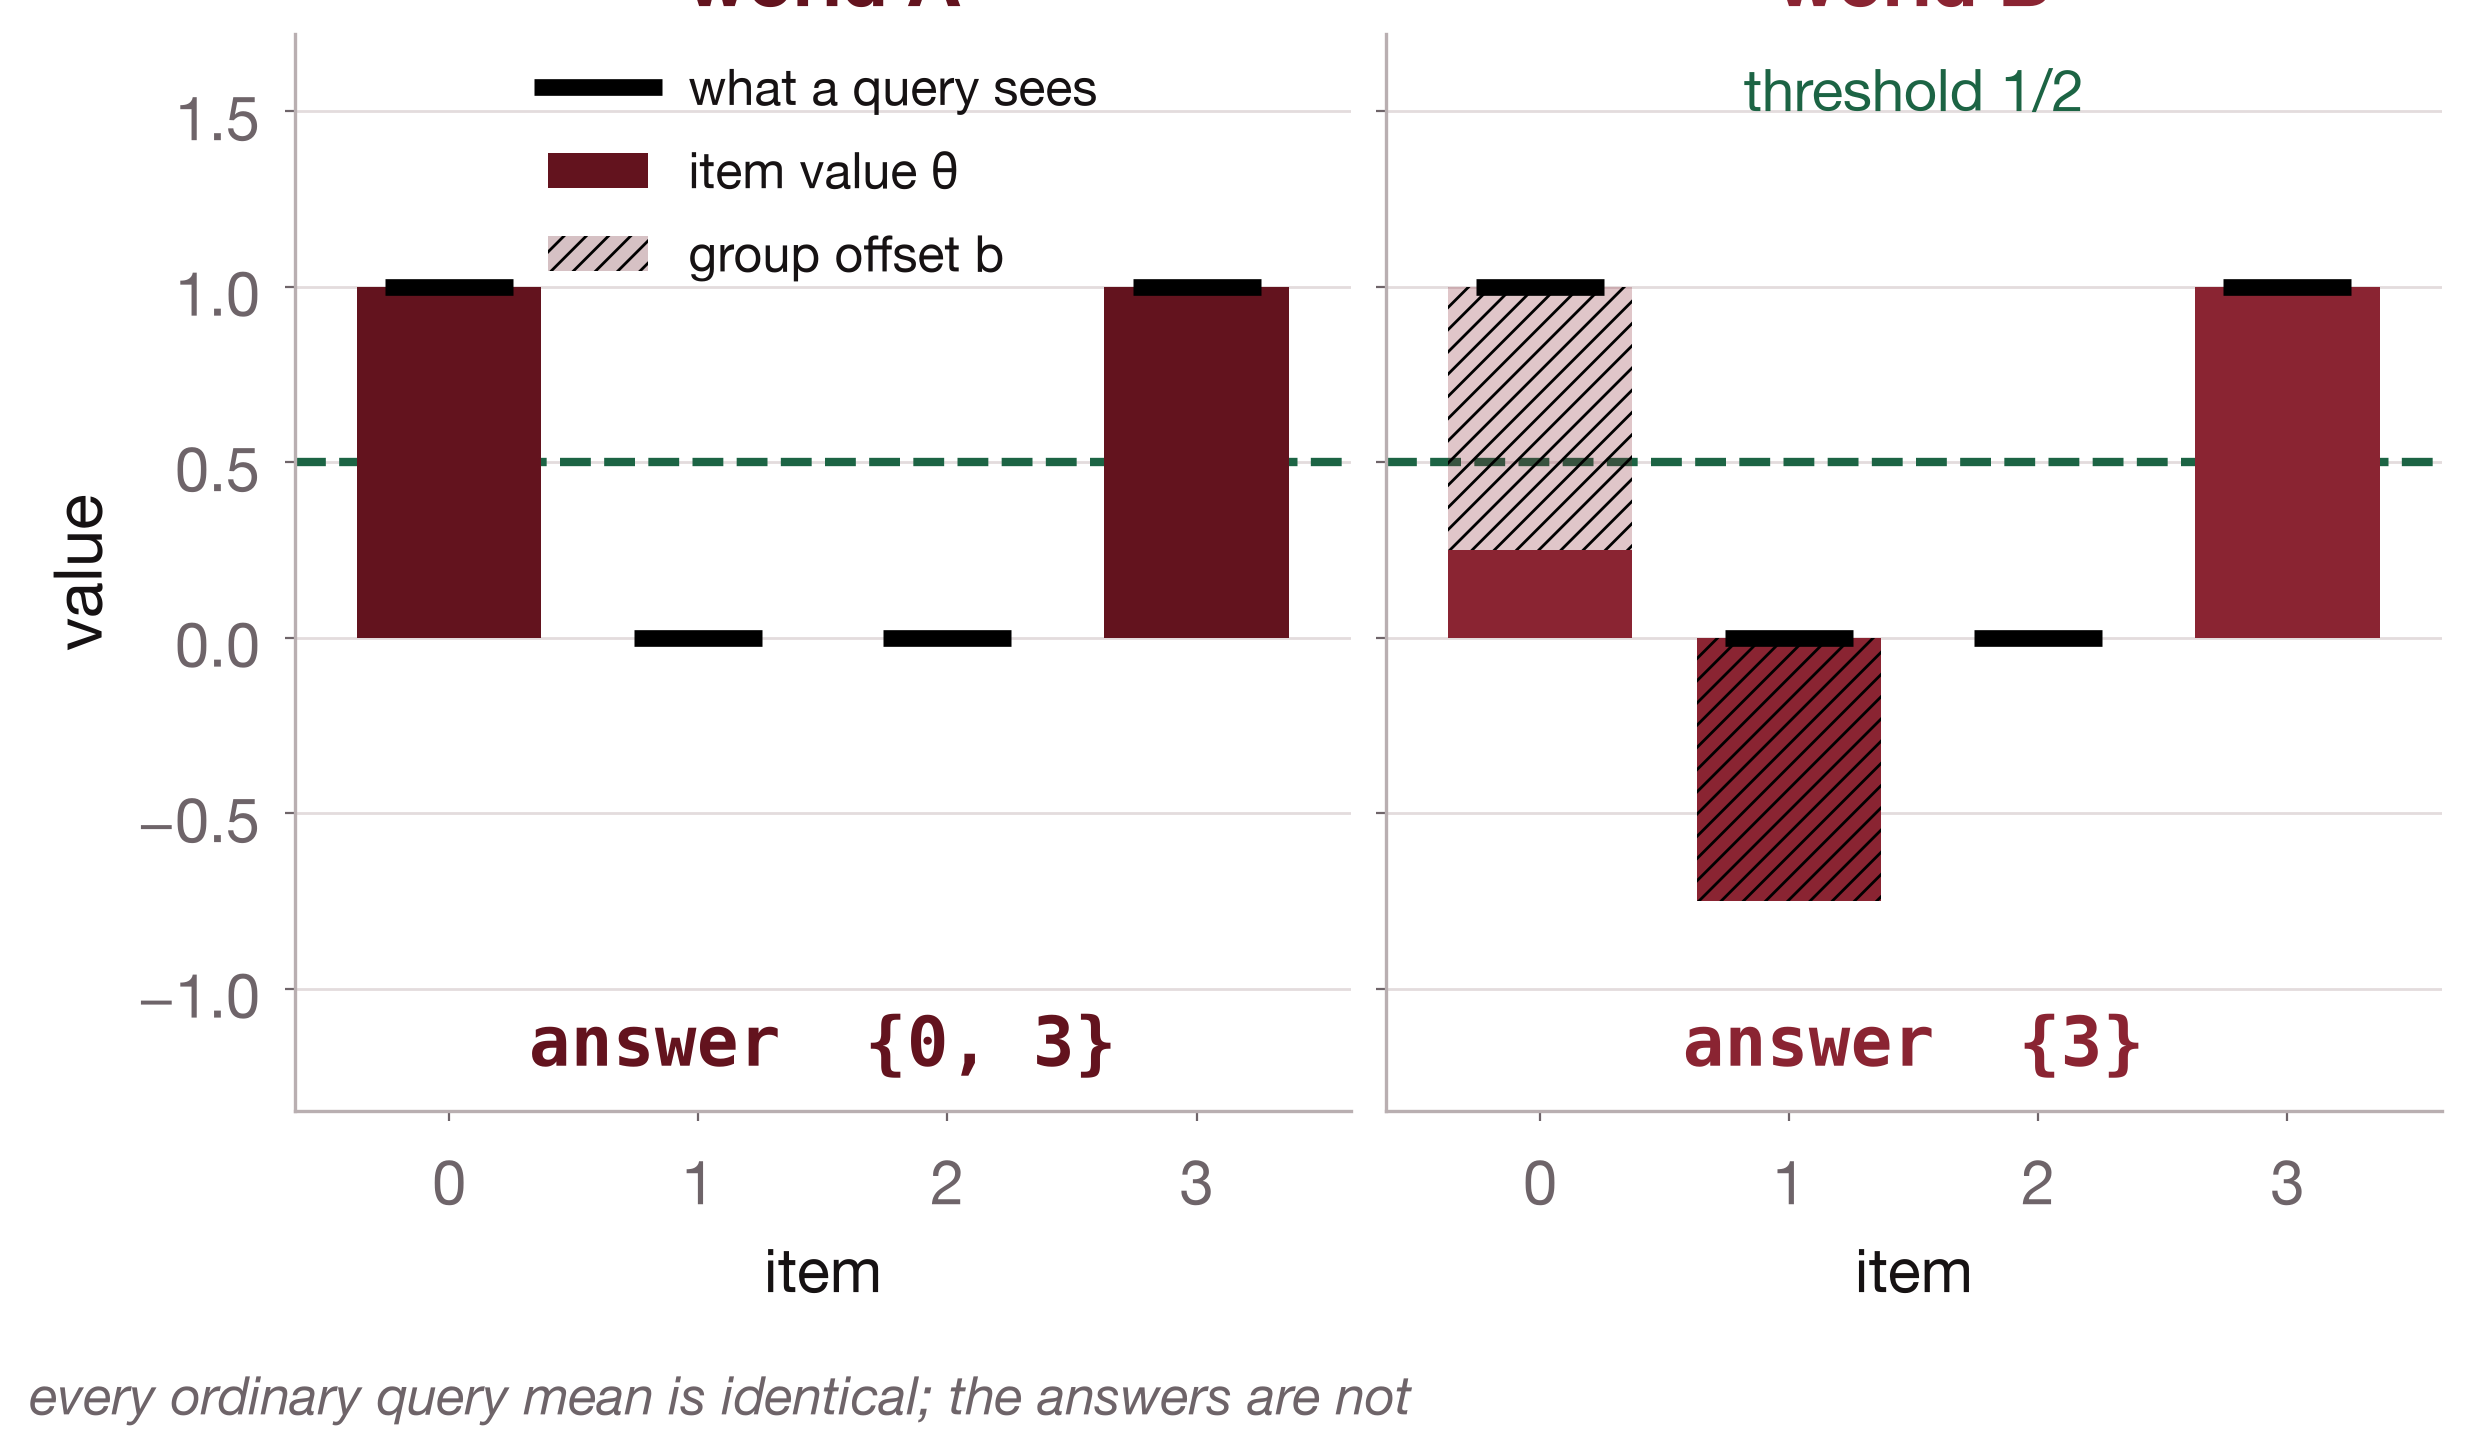
\includegraphics[width=\columnwidth]{master_fig4_witness.png}
\caption{The witness of Theorem~\ref{thm:dichotomy}. Left: the two worlds differ at item
$0$, whose value crosses the threshold $\tau=\tfrac12$ in one world and not in the other,
so the answers are different sets. Right: the observable means $\theta_{i}+b_{g(i)}$ agree
at every one of the four items, so every ordinary query has the same distribution in both
worlds. The construction pays the shift back through the group offset, which is the only
channel through which an ordinary query can be blinded.}
\label{fig:witness}
\end{figure}

\subsection{Why an exact witness rather than an asymptotic argument}

An asymptotic statement---that discrimination becomes hard as some parameter degenerates---
would be weaker in two respects. It would leave open whether the difficulty is an artefact
of the limit, and it would give the practitioner no instance to test an implementation
against. The construction above is neither: it is four items, two groups and four rational
numbers, and it is checked by the theorem prover as a closed arithmetic identity with no
real-analytic content. An implementation that claims to solve the design problem can be run
on it directly, and must return either a calibration query or a failure.

\section{Profiling the group offset}
\label{sec:profile}

With a calibration query available, the unknown offset can be eliminated from the energy.

\begin{theorem}[Profiled information]
\label{thm:profile}
For $a,b>0$ and $\Delta\in\mathbb{R}$,
\begin{equation}
\inf_{t\in\mathbb{R}}\left[\frac{a(\Delta-t)^{2}}{2}+\frac{b\,t^{2}}{2}\right]
\;=\;\frac{a\,b\,\Delta^{2}}{2(a+b)}
\;=\;\frac{\Delta^{2}}{2\left(\frac{1}{a}+\frac{1}{b}\right)} ,
\label{eq:profile}
\end{equation}
and the infimum is attained at $t^{*}=a\Delta/(a+b)$.
\end{theorem}

\begin{proof}
Write $f(t)=\tfrac12\bigl(a(\Delta-t)^{2}+bt^{2}\bigr)$. Completing the square,
\begin{equation}
f(t)=\frac{a+b}{2}\Bigl(t-\frac{a\Delta}{a+b}\Bigr)^{2}+\frac{ab\Delta^{2}}{2(a+b)},
\end{equation}
which is at least the second term for every $t$, with equality exactly at $t=t^{*}$. The
second equality in \eqref{eq:profile} is $ab/(a+b)=1/(1/a+1/b)$.
\end{proof}

\leanbox{\lean{profiled\_information}, \lean{profiled\_information\_form} in
\lean{LeanMasterCalibrationLawV1}}

Both halves are proved separately in the formalisation: the inequality for every $t$, and
the value at the minimiser. The harmonic form on the right of \eqref{eq:profile} is the
shape that propagates through the remainder of the argument, and per
Section~\ref{sec:related} that shape belongs to prior work. What is new is that the two
precisions being combined belong to two differently \emph{priced} query types, which is
what turns Section~\ref{sec:groupcost} into a statement about cost rather than about
information.

\section{The cost of one group}
\label{sec:groupcost}

A group required to deliver profiled information $h$ must satisfy the information
constraint $h(x+z)\le xz$, where $x$ and $z$ are the ordinary and control sample counts
allocated to it. The cost of that allocation, at prices $m$ and $\kappa$, is
$m\,x+\kappa\,z$.

\begin{theorem}[Group cost, lower bound]
\label{thm:grouplower}
Let $h,x,z>0$ and $s_{m},s_{\kappa}>0$ satisfy $h(x+z)\le xz$. Then
\begin{equation}
h\,(s_{m}+s_{\kappa})^{2} \;\le\; s_{m}^{2}\,x + s_{\kappa}^{2}\,z .
\label{eq:grouplower}
\end{equation}
\end{theorem}

\begin{proof}
By Cauchy--Schwarz applied to $(s_{m}x-s_{\kappa}z)^{2}\ge 0$,
\begin{equation}
(s_{m}+s_{\kappa})^{2}\,xz \;\le\; \bigl(s_{m}^{2}x+s_{\kappa}^{2}z\bigr)(x+z).
\label{eq:cs}
\end{equation}
The hypothesis gives $h(x+z)\le xz$, so multiplying by $(s_{m}+s_{\kappa})^{2}>0$,
\begin{equation}
h\,(s_{m}+s_{\kappa})^{2}(x+z) \;\le\; (s_{m}+s_{\kappa})^{2}\,xz .
\end{equation}
Chaining with \eqref{eq:cs} and dividing by $x+z>0$ yields \eqref{eq:grouplower}.
\end{proof}

\leanbox{\lean{group\_cost\_lower} in \lean{LeanMasterCalibrationLawV1}}

No optimiser is run and no multiplier theorem is invoked; the inequality is elementary and
holds for every feasible pair $(x,z)$. A lower bound alone, however, leaves the constant
unidentified, and the next result removes that gap.

\begin{theorem}[Group cost, attained]
\label{thm:groupattained}
For $h,s_{m},s_{\kappa}>0$ set
\begin{equation}
x^{\star}=\frac{h(s_{m}+s_{\kappa})}{s_{m}},
\qquad
z^{\star}=\frac{h(s_{m}+s_{\kappa})}{s_{\kappa}} .
\label{eq:groupsplit}
\end{equation}
Then $s_{m}^{2}x^{\star}+s_{\kappa}^{2}z^{\star}=h(s_{m}+s_{\kappa})^{2}$ and the
information constraint holds with equality, $h(x^{\star}+z^{\star})=x^{\star}z^{\star}$.
\end{theorem}

\begin{proof}
Direct substitution. For the cost,
$s_{m}^{2}x^{\star}+s_{\kappa}^{2}z^{\star}
= h(s_{m}+s_{\kappa})(s_{m}+s_{\kappa})=h(s_{m}+s_{\kappa})^{2}$.
For the constraint, $x^{\star}+z^{\star}=h(s_{m}+s_{\kappa})^{2}/(s_{m}s_{\kappa})$ and
$x^{\star}z^{\star}=h^{2}(s_{m}+s_{\kappa})^{2}/(s_{m}s_{\kappa})$, so multiplying the
former by $h$ gives the latter.
\end{proof}

\leanbox{\lean{group\_cost\_attained} in \lean{LeanMasterCalibrationLawV1}}

\begin{corollary}
\label{cor:groupprice}
With $s_{m}=\sqrt{m}$ and $s_{\kappa}=\sqrt{\kappa}$, the exact price of one unit of
profiled information in a group is $(\sqrt{m}+\sqrt{\kappa})^{2}$, and the optimal split
satisfies $z^{\star}/x^{\star}=\sqrt{m/\kappa}$.
\end{corollary}

The two query prices combine through their square roots. This is the signature of a
two-resource harmonic trade-off, and it has the practical consequence that neither type can
be dropped: as $x\to\infty$ with $z$ fixed, the constraint $h(x+z)\le xz$ forces
$h\le z$, so a group with no control precision cannot deliver information exceeding what
its control alone supports---which, by Theorem~\ref{thm:dichotomy}, may be nothing at all.

\section{The price law}
\label{sec:law}

\begin{theorem}[Upper bound over every design]
\label{thm:upper}
Let $x_{g},z_{g}>0$ for $g=1,\dots,K$, let $s_{m},s_{\kappa},\Delta,V>0$, and suppose the
unit budget \eqref{eq:budget} holds together with the per-group information requirement
\begin{equation}
\frac{2V}{\Delta^{2}}\,(x_{g}+z_{g}) \;\le\; x_{g}z_{g}
\qquad\text{for every } g .
\label{eq:inforeq}
\end{equation}
Then
\begin{equation}
V \;\le\; \frac{\Delta^{2}}{2K\,(s_{m}+s_{\kappa})^{2}} .
\label{eq:upper}
\end{equation}
\end{theorem}

\begin{proof}
Put $h=2V/\Delta^{2}>0$. Hypothesis \eqref{eq:inforeq} is exactly $h(x_{g}+z_{g})\le
x_{g}z_{g}$, so Theorem~\ref{thm:grouplower} applies to each group and gives
$h(s_{m}+s_{\kappa})^{2}\le s_{m}^{2}x_{g}+s_{\kappa}^{2}z_{g}$. Summing over $g$,
\begin{equation}
K\,h\,(s_{m}+s_{\kappa})^{2}
\;\le\;\sum_{g}\bigl(s_{m}^{2}x_{g}+s_{\kappa}^{2}z_{g}\bigr)\;\le\;1,
\end{equation}
the last step by the budget \eqref{eq:budget}. Substituting $h=2V/\Delta^{2}$ and
rearranging gives \eqref{eq:upper}.
\end{proof}

\leanbox{\lean{calibration\_rate\_upper} in \lean{LeanMasterCalibrationLawV1}}

The statement quantifies over \emph{every} unit-budget design satisfying
\eqref{eq:inforeq}, not over a parametric family, so no design escapes it.

\begin{theorem}[The bound is attained]
\label{thm:attained}
The symmetric design allocating \eqref{eq:groupsplit} to each of the $K$ groups, with
$h=1/\bigl(K(s_{m}+s_{\kappa})^{2}\bigr)$, satisfies the budget with equality and attains
the value in \eqref{eq:upper}. Consequently
\begin{equation}
\Gamma^{*} \;=\; \frac{\Delta^{2}}{2K\,(\sqrt{m}+\sqrt{\kappa})^{2}} .
\end{equation}
\end{theorem}

\begin{proof}
By Theorem~\ref{thm:groupattained} each group spends exactly $h(s_{m}+s_{\kappa})^{2}$, so
the total spend is $Kh(s_{m}+s_{\kappa})^{2}=1$ by the choice of $h$, and the information
constraint holds with equality in each group. The value delivered is
$V=h\Delta^{2}/2=\Delta^{2}/\bigl(2K(s_{m}+s_{\kappa})^{2}\bigr)$, which is the right-hand
side of \eqref{eq:upper}. Together with Theorem~\ref{thm:upper} this is an identity.
\end{proof}

\leanbox{\lean{calibration\_rate\_attained} in \lean{LeanMasterCalibrationLawV1}}

\subsection{Reading the law}

Two limits follow immediately and carry the practical content.

\begin{corollary}[Free calibration]
As $\kappa\to0$, $\Gamma^{*}\to\Delta^{2}/(2Km)$: the cost reduces to that of the ordinary
queries alone.
\end{corollary}

\begin{corollary}[Expensive calibration]
As $\kappa\to\infty$, $\Gamma^{*}\asymp\Delta^{2}/(2K\kappa)$: the calibration query
dominates the budget and the group size becomes irrelevant.
\end{corollary}

\begin{corollary}[Crossover]
\label{cor:crossover}
At $\kappa=m$ the two square roots in \eqref{eq:pricelaw} are equal, and by
Corollary~\ref{cor:groupprice} the optimal split satisfies $z^{\star}=x^{\star}$: each
query type consumes exactly half of each group's budget.
\end{corollary}

Corollary~\ref{cor:crossover} gives the practitioner a concrete rule. Below $\kappa=m$,
ordinary sampling dominates the budget and calibration is cheap insurance; above it, the
calibration query is the binding cost and the group size $m$ is what must be reconsidered.

\begin{figure}[htbp]
\centering
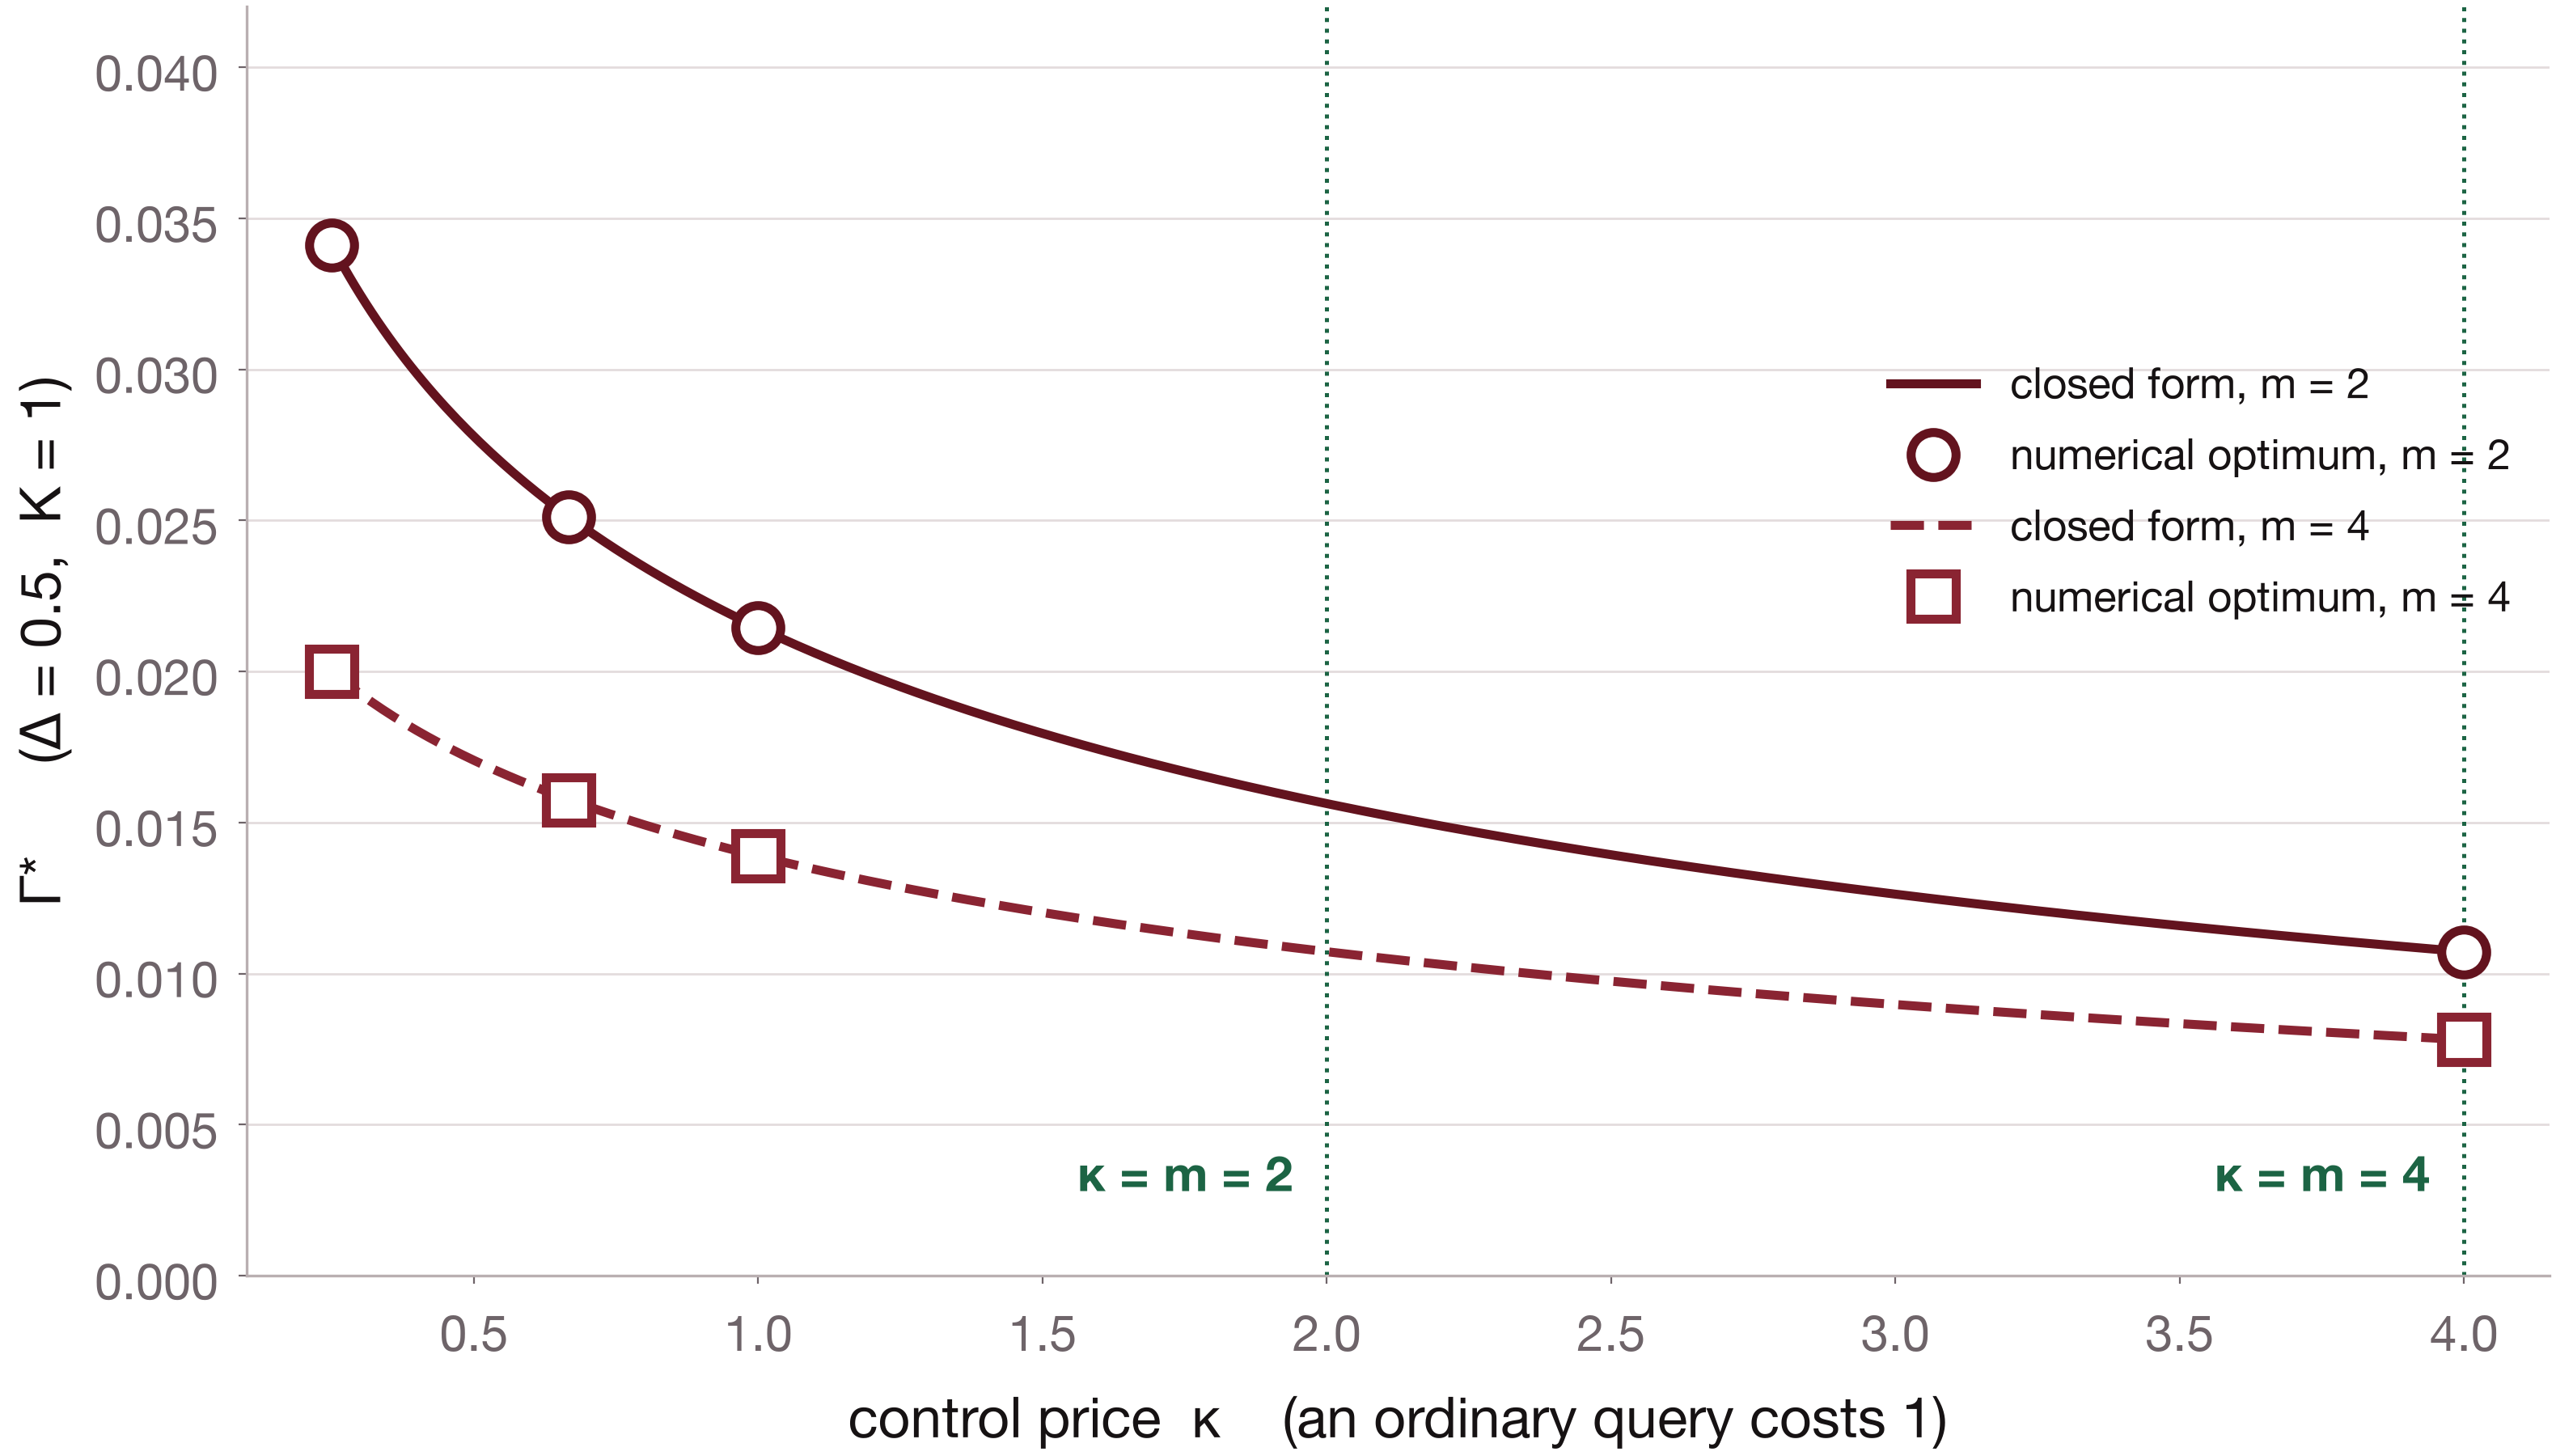
\includegraphics[width=\columnwidth]{master_fig1_rate.png}
\caption{The closed form \eqref{eq:pricelaw} against an independent bisection optimiser
over the same feasible set, across the parameter grid. The curves coincide to
floating-point precision at every cell; the largest relative gap in the sweep is
$2.5\times10^{-16}$. The decay in $\kappa$ is the $1/(\sqrt{m}+\sqrt{\kappa})^{2}$ envelope,
not a fitted rate.}
\label{fig:rate}
\end{figure}

\subsection{Constructing the optimal design}

The proof of Theorem~\ref{thm:attained} is constructive, and the construction is short
enough to state in full.

\begin{enumerate}
\item Compute $s_{m}=\sqrt{m}$ and $s_{\kappa}=\sqrt{\kappa}$ from the group size and the
calibration price.
\item Set the per-group information target
$h=1/\bigl(K(s_{m}+s_{\kappa})^{2}\bigr)$, which is the largest value the unit budget
supports across $K$ groups.
\item In every group allocate
$x^{\star}=h(s_{m}+s_{\kappa})/s_{m}$ ordinary samples and
$z^{\star}=h(s_{m}+s_{\kappa})/s_{\kappa}$ control samples, as in \eqref{eq:groupsplit}.
\item Report $\Gamma^{*}=h\Delta^{2}/2$.
\end{enumerate}

No iteration, no matrix inversion and no numerical optimiser appears. Step~3 spends exactly
$h(s_{m}+s_{\kappa})^{2}$ per group by Theorem~\ref{thm:groupattained}, so step~2 makes the
total spend exactly one, and the budget is saturated rather than approached. The ratio
$z^{\star}/x^{\star}=\sqrt{m/\kappa}$ is independent of $K$, of $h$ and of $\Delta$: the
\emph{shape} of the optimal design within a group depends only on the two prices, and the
scale is what the budget and the group count determine.

\subsection{Why the upper bound has to quantify over all designs}

A weaker theorem would fix a parametric family---symmetric designs, say, or designs with a
single control per group---and optimise inside it. Such a statement cannot rule out that a
cleverer family does better, and in a paper whose point is that a query type is
\emph{mandatory} that gap would be fatal: an opponent could always answer that some
unexamined design avoids the calibration query. Theorem~\ref{thm:upper} closes that route.
Its hypotheses are the budget and the per-group information requirement, both of which any
design delivering value $V$ must satisfy; nothing about the design's structure is assumed.
The route from a per-group inequality to a global one is the summation step, and it is
legitimate precisely because Theorem~\ref{thm:grouplower} holds for \emph{every} feasible
pair $(x_{g},z_{g})$ rather than for an optimal one.

\section{The anchor is mandatory on an instance}
\label{sec:anchor}

Theorem~\ref{thm:dichotomy} shows that a group can be blind. The companion statement is
that on a \emph{specific} instance no anchor-free design matches an anchored one, with both
sides certified in exact rational arithmetic.

\begin{theorem}[Anchor necessity, certified]
\label{thm:anchor}
On the instance of Section~\ref{sec:anchorinstance}, every anchor-free feasible design has
value at most $U_{0}=\tfrac18$, and this cap is attained. An explicit anchored design with
budget $\tfrac{9}{20}+\tfrac{9}{20}+\tfrac{1}{10}\cdot 1 = 1$ attains
$L_{1}=\tfrac{261}{1520}$. Since $\tfrac18 < \tfrac{261}{1520}$, the anchor is mandatory on
this instance.
\end{theorem}

\leanbox{\lean{anchorFree\_le}, \lean{anchorFree\_attained}, \lean{anchored\_value},
\lean{gap\_positive}, \lean{anchor\_is\_mandatory} in \lean{LeanMasterAnchorInstanceV1};
\lean{anchor\_mandatory} in \lean{LeanMasterAnchorCertificateV1}}

\subsection{The instance and the certificate}
\label{sec:anchorinstance}

The cap on anchor-free designs is a dual certificate valid for \emph{every} such design,
including those placing mass anywhere in the feasible set, and it is attained, so it is
tight rather than merely valid. The anchored value comes from an explicit design whose
budget is exhibited above. Numerically $\tfrac18=0.125$ and
$\tfrac{261}{1520}\approx0.171710$, a gap of $37.4\%$.

The formal statement \lean{anchor\_mandatory} is given for an \emph{abstract} design type.
No optimality of the anchored design is assumed: the theorem says only that an upper
certificate for one class is strictly below an achieved value in another, which is the
minimal statement that establishes necessity.

\begin{remark}
Theorem~\ref{thm:anchor} certifies one instance. It proves that anchor-free designs
\emph{can} be strictly beaten, not that they always are.
\end{remark}

\begin{figure}[htbp]
\centering
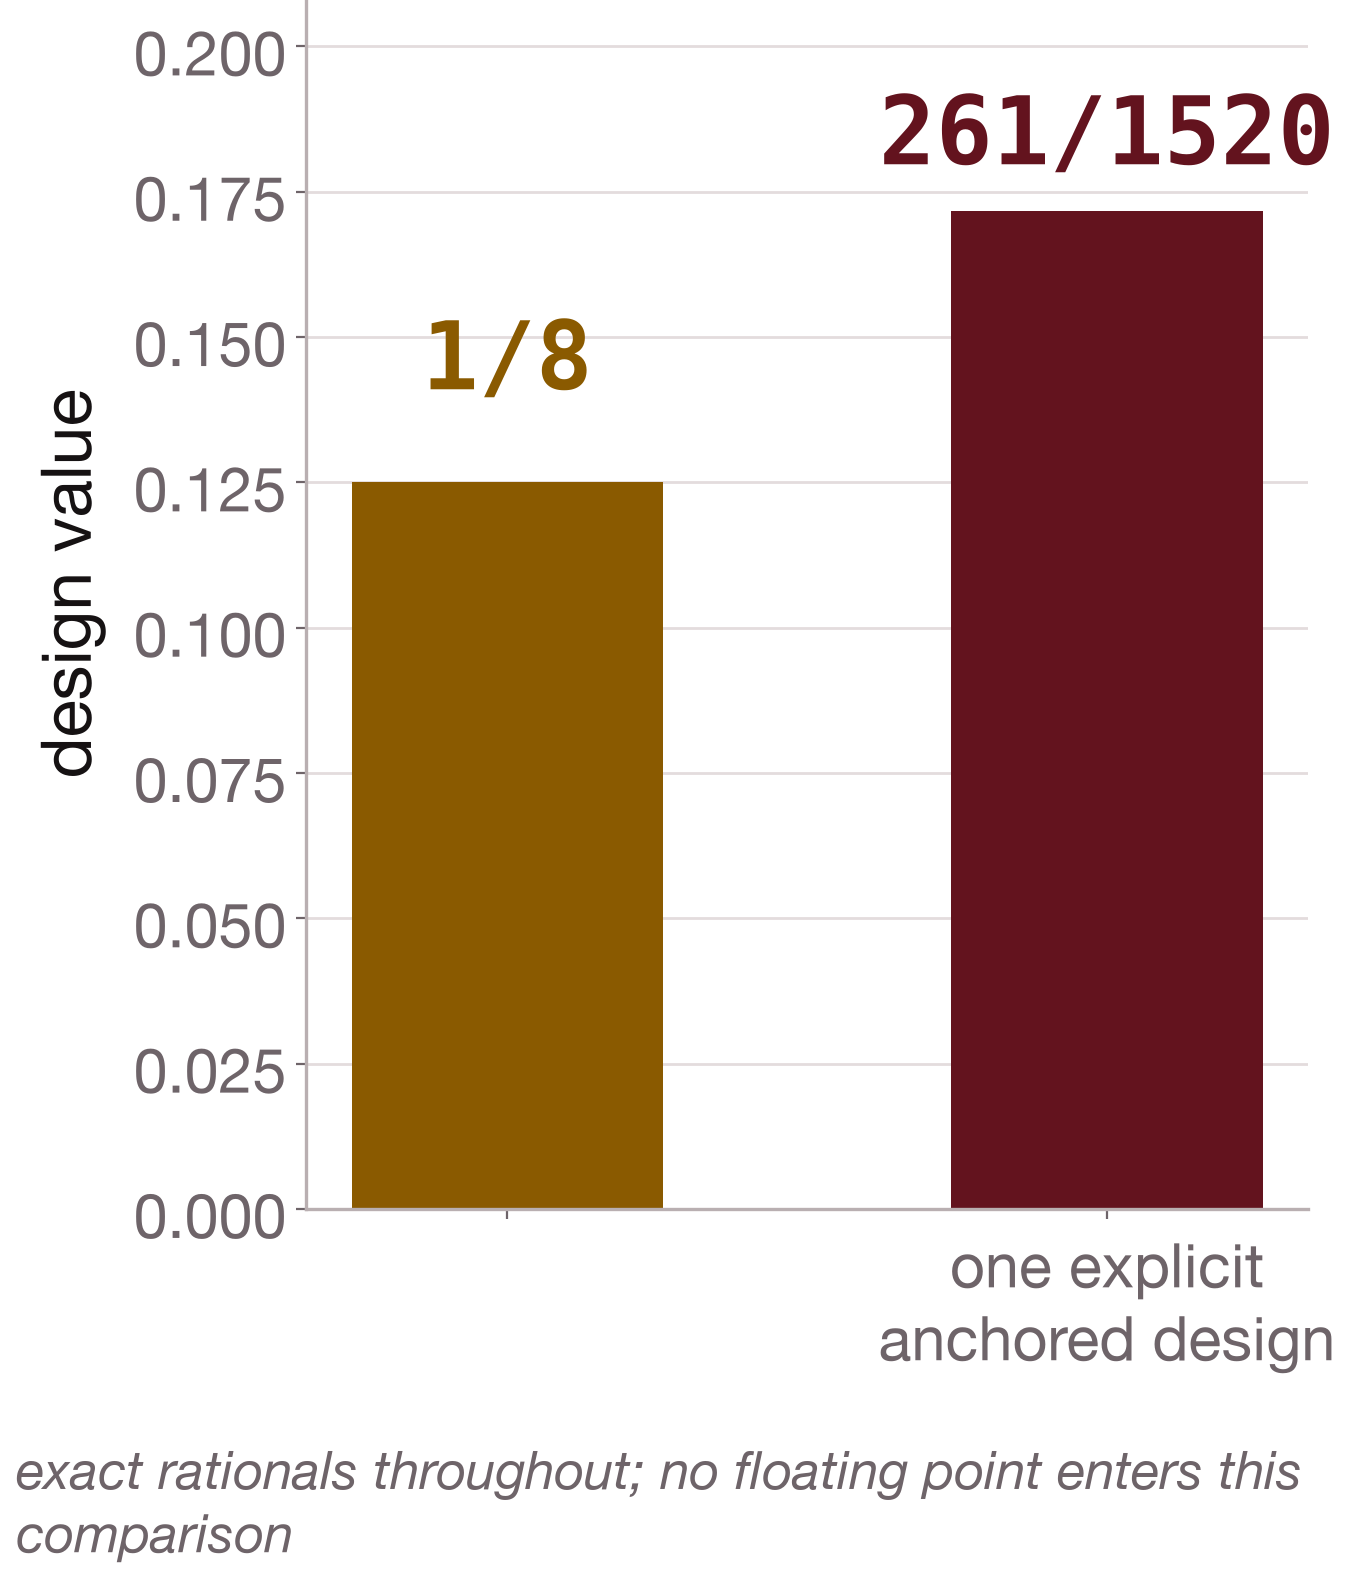
\includegraphics[width=\columnwidth]{master_fig3_anchor.png}
\caption{The certified gap of Theorem~\ref{thm:anchor}. The anchor-free class is capped at
$\tfrac18$ by a dual certificate valid for every member of the class, and that cap is
attained, so it cannot be improved. An explicit anchored design reaches $\tfrac{261}{1520}$.
Both numbers are exact rationals verified by the theorem prover, so the $37.4\%$ gap is a
certificate rather than a measurement.}
\label{fig:anchor}
\end{figure}

\subsection{Why the certificate is stated for an abstract design type}

It would be easy, and misleading, to prove the anchored design optimal on this instance and
report the gap to the optimum. That statement would require an optimality argument for the
anchored side, and any weakness in it would propagate into the necessity claim. The
formalisation avoids the dependency: \lean{anchor\_mandatory} takes an abstract type of
designs, a predicate marking the anchor-free ones, an upper certificate $U_{0}$ for that
predicate, and an achieved value $L_{1}$ for some design, and concludes strict
separation from $U_{0}<L_{1}$ alone. The instance then supplies $U_{0}=\tfrac18$ and
$L_{1}=\tfrac{261}{1520}$. Necessity therefore rests on one inequality between two
rationals, and on nothing about how either side was found.

\section{Gain factorisation}
\label{sec:gain}

The $K$-group sum in Theorem~\ref{thm:upper} is assembled from per-group statements. Two
structural facts make that assembly legitimate without a separate convexity argument.

\begin{lemma}[Hadamard square]
\label{lem:hadamard}
The entrywise square of a width-$r$ product is a product of width $r^{2}$; in particular
$(c_{k}d_{k})^{2}=c_{k}^{2}d_{k}^{2}$ for every $k$.
\end{lemma}

\begin{lemma}[Slack law]
\label{lem:slack}
The minimum after a perturbation is attained on the active set, so inactive constraints may
be dropped without changing the value.
\end{lemma}

\leanbox{\lean{hadamard\_square\_factor}, \lean{hadamard\_factor\_symm},
\lean{min\_attained\_on\_active}, \lean{inactive\_dropped} in
\lean{LeanMasterGainFactorizationV1}}

\section{Formal verification}
\label{sec:verification}

Every theorem stated above is machine-checked in Lean~4, toolchain
\texttt{leanprover/lean4:v4.34.0-rc2} against mathlib revision \texttt{1f495c61}.

\subsection{Acceptance contract}

A module counts as accepted only when all six of the following hold: the compiler exits
zero with no errors; the source hash is unchanged \emph{across} the compile, so the file
checked is the file on disk; the compiled artifact is newer than its source; at least one
\texttt{\#print axioms} directive is present; the axiom set of every audited declaration
lies within $\{\textsf{propext},\textsf{Classical.choice},\textsf{Quot.sound}\}$; and no
\texttt{sorry} appears anywhere in the file.

\subsection{Modules}

\begin{table}[htbp]
\caption{Lean modules behind the results of this paper.}
\label{tab:modules}
\centering
\begin{tabular}{@{}lrr@{}}
\toprule
Module & Audited & Results \\
\midrule
\lean{LeanMasterCalibrationLawV1}   & 10 & Thms \ref{thm:dichotomy}--\ref{thm:attained} \\
\lean{LeanMasterAnchorCertificateV1} &  6 & Thm \ref{thm:anchor} \\
\lean{LeanMasterAnchorInstanceV1}    &  8 & Thm \ref{thm:anchor} \\
\lean{LeanMasterGainFactorizationV1} &  5 & Lems \ref{lem:hadamard}, \ref{lem:slack} \\
\midrule
Total                                & 29 & \\
\bottomrule
\end{tabular}
\end{table}

\subsection{The statements as they are checked}

Formal-methods claims are only as strong as the statements actually proved, so the two
load-bearing ones are reproduced exactly as the prover has them.

\begin{figure}[htbp]
\footnotesize
\hrule\vspace{4pt}
\begin{tabbing}
\quad\=\quad\=\kill
\lean{theorem group\_cost\_lower (h x z sm sk : $\mathbb{R}$)} \\
\> \lean{(hsm : 0 < sm) (hsk : 0 < sk) (hh : 0 < h)} \\
\> \lean{(hx : 0 < x) (hz : 0 < z)} \\
\> \lean{(hinfo : h * (x + z) $\le$ x * z) :} \\
\> \lean{h * (sm + sk)\^{}2 $\le$ sm\^{}2 * x + sk\^{}2 * z} \\[6pt]
\lean{theorem calibration\_rate\_upper} \\
\> \lean{(sm sk D V : $\mathbb{R}$) (x z : Fin K $\to$ $\mathbb{R}$)} \\
\> \lean{(hsm : 0 < sm) (hsk : 0 < sk) (hD : 0 < D)} \\
\> \lean{(hV : 0 < V) (hK : 0 < K)} \\
\> \lean{(hx : $\forall$ g, 0 < x g) (hz : $\forall$ g, 0 < z g)} \\
\> \lean{(hbudget : $\sum$ g, (sm\^{}2 * x g + sk\^{}2 * z g) $\le$ 1)} \\
\> \lean{(hinfo : $\forall$ g, 2*V/D\^{}2 * (x g + z g) $\le$ x g * z g) :} \\
\> \lean{V $\le$ D\^{}2 / (2 * (K : $\mathbb{R}$) * (sm + sk)\^{}2)}
\end{tabbing}
\vspace{-4pt}\hrule
\caption{The two statements carrying the price law, as checked ($D$ is the paper's
$\Delta$; $K$ is a section variable). The upper bound quantifies over arbitrary allocation
functions \lean{x z : Fin K $\to$ $\mathbb{R}$} constrained only by the budget and the
information requirement; no structure on the design is assumed and no parametric family is
fixed.}
\label{fig:statements}
\end{figure}

Three details of Fig.~\ref{fig:statements} are worth naming. The hypothesis \lean{hinfo} is
an inequality, not an equality, so the lower bound covers designs that over-deliver
information as well as those that meet the requirement exactly. The budget
\lean{hbudget} is likewise an inequality, so designs that underspend are included. And $V$
is universally quantified rather than defined as a supremum, which is what makes the
conclusion a bound on every achievable value rather than a statement about a particular
optimum.

\subsection{What the paper derives rather than cites}

Four displayed results carry no \lean{leanbox} because the paper obtains them itself from
the checked ones, and they are listed here rather than left to inference:
Corollary~\ref{cor:groupprice} (substituting $s_{m}=\sqrt{m}$, $s_{\kappa}=\sqrt{\kappa}$
into Theorem~\ref{thm:groupattained}), the two limits $\kappa\to0$ and $\kappa\to\infty$,
and Corollary~\ref{cor:crossover} (setting $\kappa=m$). Each is one line of algebra from a
machine-checked statement. The likelihood derivation \eqref{eq:llr} and the
Cauchy--Schwarz step \eqref{eq:cs} are likewise worked out in the paper; the identity they
lead to is \lean{profiled\_information} and \lean{group\_cost\_lower} respectively, both
checked.

\subsection{Evidence per step of the argument}

Table~\ref{tab:inventory} records, for each step of the development, the declarations the
step cites and the module they live in. It is included because a formal-methods claim is
not checkable from a count of theorems alone: the question is always which named result
carries which step.

\begin{table}[htbp]
\caption{Evidence per step. All cited declarations are axiom-audited.}
\label{tab:inventory}
\centering
\footnotesize
\setlength{\tabcolsep}{3pt}
\begin{tabular}{@{}llr@{}}
\toprule
Step & Cited declarations & Aud. \\
\midrule
Dichotomy, Thm~\ref{thm:dichotomy}
  & \lean{hidden\_shift\_means} & 10 \\
  & \lean{hidden\_shift\_answers\_differ} & \\
  & \lean{hidden\_shift\_witness} & \\
Profiling, Thm~\ref{thm:profile}
  & \lean{profiled\_information} & 10 \\
  & \lean{profiled\_information\_form} & \\
Group lower, Thm~\ref{thm:grouplower}
  & \lean{group\_cost\_lower} & 10 \\
Group att., Thm~\ref{thm:groupattained}
  & \lean{group\_cost\_attained} & 10 \\
Upper bd., Thm~\ref{thm:upper}
  & \lean{calibration\_rate\_upper} & 10 \\
Attained, Thm~\ref{thm:attained}
  & \lean{calibration\_rate\_attained} & 10 \\
Anchor cap, Thm~\ref{thm:anchor}
  & \lean{anchorFree\_le} & 8 \\
  & \lean{anchorFree\_attained} & \\
Anchor val., Thm~\ref{thm:anchor}
  & \lean{anchored\_value} & 8 \\
  & \lean{gap\_positive} & \\
Necessity, Thm~\ref{thm:anchor}
  & \lean{anchor\_mandatory} & 6 \\
Factorise, Lem~\ref{lem:hadamard}
  & \lean{hadamard\_square\_factor} & 5 \\
Slack, Lem~\ref{lem:slack}
  & \lean{min\_attained\_on\_active} & 5 \\
  & \lean{inactive\_dropped} & \\
\bottomrule
\end{tabular}
\end{table}

\subsection{Scope of the formalisation}

The displayed results are the load-bearing chain, not the whole development. The MASTER
strand contains $15$ Lean source files with $122$ theorem and lemma statements, of which the
modules in Table~\ref{tab:modules} carry acceptance receipts covering $57$ audited
declarations. Across the programme of which this paper is one part: $762$ files, $7{,}199$
statements, $111$ accepted modules, $875$ audited declarations. The statements not
displayed are the arithmetic identities, positivity checks and finite-sum exchanges that
each displayed result rests on.

No module cited in this paper contains a \texttt{sorry}. Seven occurrences exist in the
wider repository, in audit scaffolding and in files named as conjectures; the overlap
between the cited set and the files containing them was computed and is empty.

\section{Numerical validation}
\label{sec:experiments}

The theorems above are proved, so numerical work here serves only to check the
implementation and to quantify the practical consequence. It is reported separately and
never substitutes for a proof.

\subsection{The law against an independent optimiser}

Over $32$ parameter cells spanning $K\in\{1,2,4,8\}$, $m\in\{2,4\}$ and
$\kappa\in\{\tfrac14,\tfrac23,1,4\}$, we compare the closed form \eqref{eq:pricelaw}
against an independent numerical optimum computed by bisection on the information
constraint over the same feasible set. The optimiser does not know the closed form; it is
given the budget, the constraint and nothing else.

\begin{table}[htbp]
\caption{Closed form against an independent optimiser.}
\label{tab:numeric}
\centering
\begin{tabular}{@{}lr@{}}
\toprule
Quantity & Value \\
\midrule
Parameter cells                        & 32 \\
Cells in which the two agree           & 32 \\
Largest relative gap                   & $2.5\times10^{-16}$ \\
Cells where the optimiser exceeds the form & 0 \\
\bottomrule
\end{tabular}
\end{table}

The last row is the informative one. An upper bound is falsified by a numerical optimum
that exceeds it, and none does; the remaining rows only confirm that the implementation and
the algebra describe the same object. Per-cell values are given in Table~\ref{tab:cells},
which also carries the uniform baseline discussed next.

\subsection{Baselines: the cost of a missing query type}

Over the same $32$ cells we evaluate three baselines against the analytic optimum. Removing
all calibration queries, and removing a single one, both return \emph{exactly} zero. This
is not a small number and not a solver failure: the configuration is the witness of
Theorem~\ref{thm:dichotomy}, and unidentifiability is detected before any solver is called.
A uniform design that retains all calibration queries but splits each group's budget
evenly reaches $73.5$--$100\%$ of the optimum, with the worst case at the extreme of the
$\kappa$ range where the optimal split is most lopsided.

\begin{table}[htbp]
\caption{Baselines as a fraction of the analytic optimum, 32 cells.}
\label{tab:baselines}
\centering
\begin{tabular}{@{}lr@{}}
\toprule
Baseline & Fraction of optimum \\
\midrule
No calibration queries        & $0$ (unidentifiable) \\
One calibration query missing & $0$ (unidentifiable) \\
Uniform, all controls         & $0.735$--$1.000$ \\
Optimal design                & $1.000$ \\
\bottomrule
\end{tabular}
\end{table}

\begin{figure}[htbp]
\centering
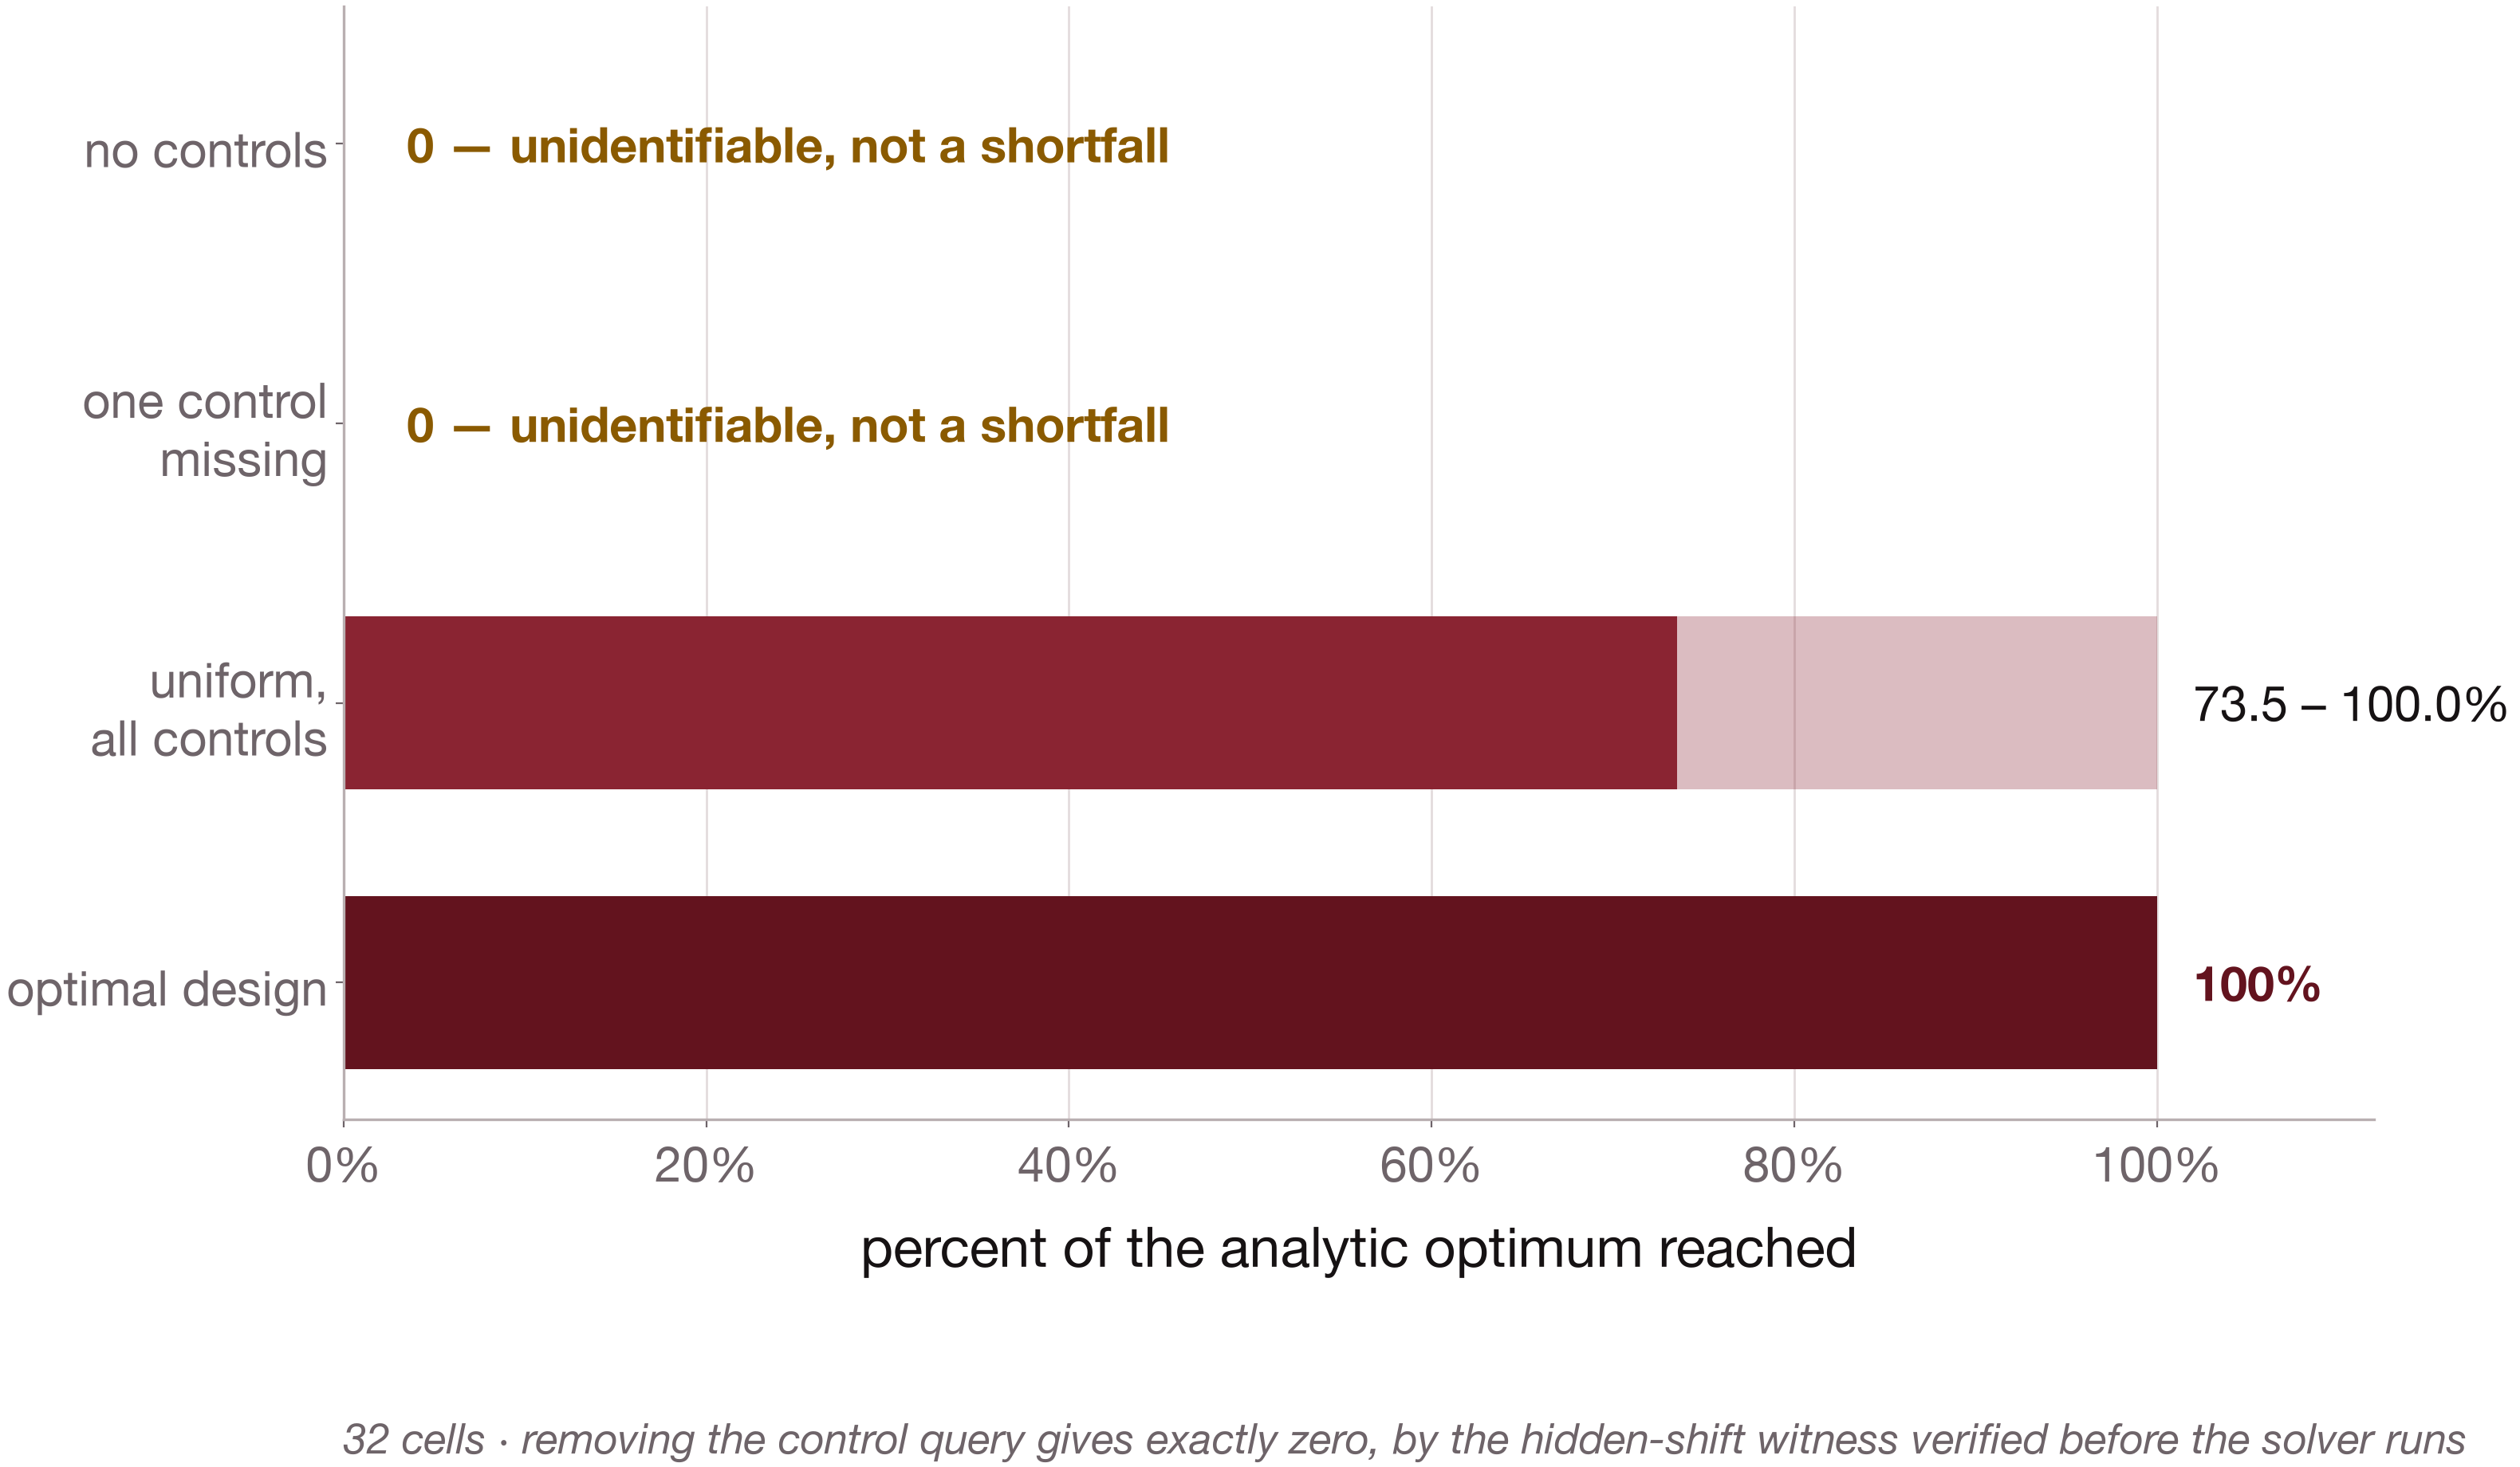
\includegraphics[width=\columnwidth]{master_fig2_baselines.png}
\caption{The asymmetry of Table~\ref{tab:baselines}. A uniform allocation that keeps every
calibration query loses a bounded fraction of the optimum. Dropping the query type returns
exactly zero on every cell, and the zero is structural: the two worlds have identical
observable means, so no allocation of ordinary samples---and no estimator built on
them---separates them.}
\label{fig:baselines}
\end{figure}

\begin{table*}[t]
\caption{The closed form \eqref{eq:pricelaw} against an independent bisection optimiser, and against the uniform baseline, on all 32 parameter cells of the grid $K\in\{1,2,4,8\}$, $m\in\{2,4\}$, $\kappa\in\{\frac14,\frac23,1,4\}$ at $\Delta=1$. The ``gap'' column is the relative difference between the closed form and the optimiser; the largest anywhere in the sweep is $2.5e-16$, i.e.\ floating-point agreement. The last column is the uniform design as a percentage of the optimum, which never falls below $73.5\%$---in sharp contrast with the two control-free baselines, which return exactly zero on every cell.}
\label{tab:cells}
\centering
\footnotesize
\setlength{\tabcolsep}{4pt}
\begin{tabular}{@{}rrrrrrrr@{\hspace{10pt}}|@{\hspace{10pt}}rrrrrrrr@{}}
\toprule
$K$ & $m$ & $\kappa$ & $\Gamma^{*}$ & bisect. & gap & unif. & \% & $K$ & $m$ & $\kappa$ & $\Gamma^{*}$ & bisect. & gap & unif. & \% \\
\midrule
1 & 2 & $\frac14$ & 0.034114 & 0.034114 & 0e+00 & 0.027778 & 81.4 & 4 & 2 & $\frac14$ & 0.008528 & 0.008528 & 2e-16 & 0.006944 & 81.4 \\
1 & 2 & $\frac23$ & 0.025120 & 0.025120 & 1e-16 & 0.023438 & 93.3 & 4 & 2 & $\frac23$ & 0.006280 & 0.006280 & 0e+00 & 0.005859 & 93.3 \\
1 & 2 & $1$ & 0.021447 & 0.021447 & 0e+00 & 0.020833 & 97.1 & 4 & 2 & $1$ & 0.005362 & 0.005362 & 0e+00 & 0.005208 & 97.1 \\
1 & 2 & $4$ & 0.010723 & 0.010723 & 2e-16 & 0.010417 & 97.1 & 4 & 2 & $4$ & 0.002681 & 0.002681 & 0e+00 & 0.002604 & 97.1 \\
1 & 4 & $\frac14$ & 0.020000 & 0.020000 & 0e+00 & 0.014706 & 73.5 & 4 & 4 & $\frac14$ & 0.005000 & 0.005000 & 2e-16 & 0.003676 & 73.5 \\
1 & 4 & $\frac23$ & 0.015758 & 0.015758 & 2e-16 & 0.013393 & 85.0 & 4 & 4 & $\frac23$ & 0.003939 & 0.003939 & 2e-16 & 0.003348 & 85.0 \\
1 & 4 & $1$ & 0.013889 & 0.013889 & 0e+00 & 0.012500 & 90.0 & 4 & 4 & $1$ & 0.003472 & 0.003472 & 0e+00 & 0.003125 & 90.0 \\
1 & 4 & $4$ & 0.007812 & 0.007812 & 1e-16 & 0.007812 & 100.0 & 4 & 4 & $4$ & 0.001953 & 0.001953 & 1e-16 & 0.001953 & 100.0 \\
2 & 2 & $\frac14$ & 0.017057 & 0.017057 & 2e-16 & 0.013889 & 81.4 & 8 & 2 & $\frac14$ & 0.004264 & 0.004264 & 2e-16 & 0.003472 & 81.4 \\
2 & 2 & $\frac23$ & 0.012560 & 0.012560 & 1e-16 & 0.011719 & 93.3 & 8 & 2 & $\frac23$ & 0.003140 & 0.003140 & 0e+00 & 0.002930 & 93.3 \\
2 & 2 & $1$ & 0.010723 & 0.010723 & 0e+00 & 0.010417 & 97.1 & 8 & 2 & $1$ & 0.002681 & 0.002681 & 0e+00 & 0.002604 & 97.1 \\
2 & 2 & $4$ & 0.005362 & 0.005362 & 0e+00 & 0.005208 & 97.1 & 8 & 2 & $4$ & 0.001340 & 0.001340 & 2e-16 & 0.001302 & 97.1 \\
2 & 4 & $\frac14$ & 0.010000 & 0.010000 & 0e+00 & 0.007353 & 73.5 & 8 & 4 & $\frac14$ & 0.002500 & 0.002500 & 0e+00 & 0.001838 & 73.5 \\
2 & 4 & $\frac23$ & 0.007879 & 0.007879 & 2e-16 & 0.006696 & 85.0 & 8 & 4 & $\frac23$ & 0.001970 & 0.001970 & 2e-16 & 0.001674 & 85.0 \\
2 & 4 & $1$ & 0.006944 & 0.006944 & 1e-16 & 0.006250 & 90.0 & 8 & 4 & $1$ & 0.001736 & 0.001736 & 2e-16 & 0.001563 & 90.0 \\
2 & 4 & $4$ & 0.003906 & 0.003906 & 1e-16 & 0.003906 & 100.0 & 8 & 4 & $4$ & 0.000977 & 0.000977 & 1e-16 & 0.000977 & 100.0 \\
\bottomrule
\end{tabular}
\end{table*}


\subsection{Reading the asymmetry}

The two halves of Table~\ref{tab:baselines} are asymmetric, and that asymmetry is the
practical message of the paper. An experimenter who allocates badly loses a bounded
fraction of the attainable information: at worst about a quarter, on this grid. An
experimenter who omits the query \emph{type} loses everything, and no amount of sampling
recovers it, because the deficiency is in the observation model rather than in the sample
size.

Efficiency and feasibility are therefore not points on a single scale. A design procedure
that treats the calibration query as one more option to be traded off against ordinary
samples will, on a configuration like the witness, allocate its entire budget to ordinary
queries---each of which is individually informative about $\theta+b$---and report a design
whose value is zero, with no indication that anything has gone wrong. The failure is silent
because every individual query in it looks useful.

\subsection{What the numerical work does and does not add}

None of the tables above proves anything: Theorems~\ref{thm:upper} and \ref{thm:attained}
are already machine-checked, and a sweep cannot strengthen a theorem. The sweeps serve two
narrower purposes. They check that the implementation used to generate the figures computes
the same quantity the theorems describe, which is a real risk in any paper pairing formal
statements with plots. And they quantify the consequence---the $73.5\%$ floor and the exact
zeros---which the theorems alone do not, because a theorem about the optimum says nothing
about how far a particular heuristic falls from it.

Consistent with this, evidence classes are kept apart throughout: statements labelled
\PROVED{} are machine-checked, \CERT{} denotes an exact rational certificate, and \NUM{}
denotes a floating-point computation. No \NUM{} result is used to support a \PROVED{} one.

\section{Discussion and scope}
\label{sec:scope}

\subsection{What the results establish}

The calibration query is not an efficiency improvement that a careful allocator could do
without. On the configurations exhibited here the attainable value is exactly zero until a
query of the new type is bought; once bought, its price is exact, matched by a lower bound,
by an upper bound over all unit-budget designs, and by an attaining design. The crossover
$\kappa=m$ converts the law into an operational rule.

\subsection{A worked example}

Suppose an array of $K=8$ sensor groups, each holding $m=4$ instruments, is to be screened
against a threshold, and a calibration run on a group costs four times an ordinary reading,
so $\kappa=4$. Then $s_{m}=2$, $s_{\kappa}=2$, and the price of one unit of profiled
information in a group is $(2+2)^{2}=16$. The budget supports
$h=1/(8\cdot 16)=1/128$ per group, and Corollary~\ref{cor:crossover} applies exactly---
$\kappa=m$---so the optimal split is even: $x^{\star}=z^{\star}=h\cdot 4/2=1/64$. Half of
every group's budget buys calibration. With $\Delta=1$ the attainable value is
$\Gamma^{*}=1/256\approx 0.0039$, which is the $K=8$, $m=4$, $\kappa=4$ row of
Table~\ref{tab:cells}.

Now suppose the calibration runs are made cheaper, $\kappa=1$. The price per unit drops to
$(2+1)^{2}=9$, the attainable value rises to $1/144\approx 0.0069$, and the split tilts:
$z^{\star}/x^{\star}=\sqrt{4/1}=2$, so calibration now takes two thirds of each group's
sample count although it still costs less in budget terms. The direction is worth noting
because it is the opposite of the intuitive one---cheaper calibration buys \emph{more}
calibration samples, not fewer, since the constraint that binds is information rather than
convenience.

Finally, suppose the calibration is dropped entirely on the grounds that $\kappa=4$ was
expensive and the instruments are nominally identical. If the group offsets are in fact
non-zero and arranged as in Section~\ref{sec:dichotomy}, the value is not $0.0039$ reduced
by some efficiency factor; it is zero, and the screening returns an answer that is wrong on
at least one item with no accompanying signal of failure.

\subsection{What the results do not establish}

\begin{enumerate}
\item \textbf{Homogeneity.} The law of Section~\ref{sec:law} assumes a common variance $v$,
a common control variance $\nu$, a common price $\kappa$ and equal gaps. Heterogeneous
$v_{i},\nu_{g},\kappa_{g}$ and unequal gaps are not covered, and the corresponding
weighted quantity is not computed here.

\item \textbf{One instance for the anchor.} Theorem~\ref{thm:anchor} certifies a single
explicit instance. It shows anchor-free designs can be strictly beaten, not that they
always are.

\item \textbf{A witness, not a characterisation.} Theorem~\ref{thm:dichotomy} exhibits two
indistinguishable worlds without characterising all such configurations.

\item \textbf{An information statement.} Everything above is an information and budget
statement. No estimator, no confidence set and no finite-sample guarantee is claimed, and
the Gaussian noise model enters only through the quadratic energy.

\item \textbf{Algebraic gain factorisation.} Lemmas~\ref{lem:hadamard} and \ref{lem:slack}
are algebraic and carry no probabilistic content.
\end{enumerate}

\subsection{Open problems}

Four questions are left open, in rough order of how tractable they look.

\emph{The heterogeneous law.} Replace the common $(v,\nu,\kappa,\Delta)$ by per-item and
per-group values. The per-group argument of Section~\ref{sec:groupcost} survives unchanged,
since Theorem~\ref{thm:grouplower} never uses homogeneity; what changes is the summation
step, where the budget is now shared between groups with different prices. The natural
conjecture is that $K(\sqrt{m}+\sqrt{\kappa})^{2}$ becomes
$\bigl(\sum_{g}(\sqrt{m_{g}}+\sqrt{\kappa_{g}})\Delta_{g}^{-1}\bigr)^{2}$-like in form, and
whether it is still exactly attainable is the question.

\emph{A test rather than a witness.} Theorem~\ref{thm:dichotomy} exhibits one blinded
configuration. A characterisation of the configurations on which the calibration query is
mandatory would let a practitioner \emph{check} an instance rather than hope it is not one
of the bad ones. The obstruction is that the property depends on the threshold $\tau$ and
on the answer map, not on the observation model alone, so the characterisation cannot be a
rank condition on the design matrix.

\emph{Partial calibration.} The results treat calibration as available or absent per group.
An intermediate regime---where a calibration query returns a linear combination of several
offsets, as a differential or a relative measurement would---interpolates between the two,
and the price in that regime is not computed here.

\emph{The meaning of the crossover.} At $\kappa=m$ the two query types consume equal shares
of each group's budget, and the value has the clean form $\Delta^{2}/(8Km)$. Whether that
coincidence has an operational reading---a point at which some qualitative property of the
optimal design changes---or is an artefact of the square-root algebra, is open.

\section{Conclusion}

We have shown that an additional \emph{type} of measurement can be a precondition rather
than an optimisation, exhibited a configuration in exact rationals where this is so, and
computed the exact price of that measurement once it is admitted. The price law
$\Gamma^{*}=\Delta^{2}/\bigl(2K(\sqrt{m}+\sqrt{\kappa})^{2}\bigr)$ is an identity: matched
on both sides and attained. Every claim is machine-checked, and the numerical work is
reported separately from the proofs it validates.

The narrower message, for a practitioner, is a checklist rather than a theory. Ask whether
the observation model sees the quantity of interest only in combination with something
unknown; if it does, ask whether any pair of worlds with different answers produces
identical observable means; and if such a pair exists, stop optimising the allocation,
because the value of every allocation is the same and it is zero.

\appendices
\section{Complete statement inventory}
\label{app:inventory}

This appendix reproduces every axiom-audited theorem and lemma in the MASTER strand\'s accepted modules---all $57$ of them, grouped by module---so that the corpus behind the paper can be read rather than counted. Each entry is a symbol-level transliteration of the Lean statement: Unicode maps to the corresponding \LaTeX{} symbol and identifiers are set upright, but no structure is rewritten and no hypothesis is dropped. What appears below is what the prover checked.

Binders are listed as the prover has them and the turnstile $\vdash$ separates them from the conclusion. Every entry carries an acceptance receipt and an axiom audit confining it to $\{\textsf{propext},\textsf{Classical.choice},\textsf{Quot.sound}\}$; none contains \texttt{sorry}.

\vspace{4pt}\noindent\rule{\columnwidth}{0.4pt}\par\vspace{2pt}
\noindent\textbf{Module \lean{LeanMasterActiveSetV1}}\par\vspace{3pt}

\noindent\textbf{A\,1}\quad\lean{anchor\_worthless\_when\_offset\_cancels}
{\footnotesize\[ \begin{aligned}[t]
&(\mathit{D} \mathit{K} \mathit{s} : \mathbb{R} ),\; (\mathit{hM} : (0:\mathbb{R} ) = 0)
\end{aligned} \]}
{\footnotesize\[ \begin{aligned}[t]
\vdash\;&\mathit{D} - (0:\mathbb{R} )^{2}/(2*(\mathit{K} + \mathit{s}))\\
&\quad = \mathit{D}
\end{aligned} \]}

\noindent\textbf{A\,2}\quad\lean{cancelling\_design\_exists}
{\footnotesize\[ \begin{aligned}[t]
&(\mathit{d₁} \mathit{d₂} : \mathbb{R} ),\; (\mathit{h₁} : 0 < \mathit{d₁}),\; (\mathit{h₂} : \mathit{d₂} <\\
&\quad 0)
\end{aligned} \]}
{\footnotesize\[ \begin{aligned}[t]
\vdash\;&\mathbf{let} \mathit{a₁}
\end{aligned} \]}

\noindent\textbf{A\,3}\quad\lean{complementary\_slackness}
{\footnotesize\[ \begin{aligned}[t]
&(\mathit{I} \mathit{lam} : \mathit{U} \to \mathbb{R} ),\; (\mathit{V} : \mathbb{R} ),\; (\mathit{hV} : \forall \mathit{u}, \mathit{V} \leq \mathit{I}\\
&\quad \mathit{u}),\; (\mathit{hl0} : \forall \mathit{u}, 0 \leq \mathit{lam} \mathit{u}),\; (\mathit{hl1} : \textstyle\sum \mathit{u}, \mathit{lam} \mathit{u} =\\
&\quad 1),\; (\mathit{htight} : \textstyle\sum \mathit{u}, \mathit{lam} \mathit{u} * \mathit{I} \mathit{u} \leq \mathit{V})
\end{aligned} \]}
{\footnotesize\[ \begin{aligned}[t]
\vdash\;&\forall \mathit{u}, 0 < \mathit{lam} \mathit{u} \to \mathit{I} \mathit{u}\\
&\quad = \mathit{V}
\end{aligned} \]}

\noindent\textbf{A\,4}\quad\lean{dual\_support\_active}
{\footnotesize\[ \begin{aligned}[t]
&(\mathit{I} \mathit{lam} : \mathit{U} \to \mathbb{R} ),\; (\mathit{V} : \mathbb{R} ),\; (\mathit{hl0} : \forall \mathit{u}, 0 \leq \mathit{lam}\\
&\quad \mathit{u}),\; (\mathit{hl1} : \textstyle\sum \mathit{u}, \mathit{lam} \mathit{u} = 1),\; (\mathit{u0} :\\
&\quad \mathit{U}),\; (\mathit{hattain} : \mathit{I} \mathit{u0} = \mathit{V}),\; (\mathit{hmin} : \forall \mathit{u}, \mathit{I} \mathit{u0} \leq \mathit{I}\\
&\quad \mathit{u}),\; (\mathit{hcap} : \textstyle\sum \mathit{u}, \mathit{lam} \mathit{u} * \mathit{I} \mathit{u} \leq \mathit{V})
\end{aligned} \]}
{\footnotesize\[ \begin{aligned}[t]
\vdash\;&\forall \mathit{u}, 0 < \mathit{lam} \mathit{u} \to \mathit{I} \mathit{u}\\
&\quad = \mathit{V}
\end{aligned} \]}

\noindent\textbf{A\,5}\quad\lean{min\_improves}
{\footnotesize\[ \begin{aligned}[t]
&(\mathit{I'} : \mathit{U} \to \mathbb{R} ),\; (\mathit{V} : \mathbb{R} ),\; (\mathit{hall} : \forall \mathit{u}, \mathit{V} < \mathit{I'}\\
&\quad \mathit{u})
\end{aligned} \]}
{\footnotesize\[ \begin{aligned}[t]
\vdash\;&\mathit{V} < (\mathit{univ} : \mathit{Finset} \mathit{U}).\mathit{inf'}\\
&\quad \mathit{univ\_{}nonempty} \mathit{I'}
\end{aligned} \]}

\noindent\textbf{A\,6}\quad\lean{one\_bad\_blocks}
{\footnotesize\[ \begin{aligned}[t]
&(\mathit{I'} : \mathit{U} \to \mathbb{R} ),\; (\mathit{V} : \mathbb{R} ),\; (\mathit{u0} :\\
&\quad \mathit{U}),\; (\mathit{hbad} : \mathit{I'} \mathit{u0} \leq \mathit{V})
\end{aligned} \]}
{\footnotesize\[ \begin{aligned}[t]
\vdash\;&(\mathit{univ} : \mathit{Finset} \mathit{U}).\mathit{inf'} \mathit{univ\_{}nonempty}\\
&\quad \mathit{I'} \leq \mathit{V}
\end{aligned} \]}

\noindent\textbf{A\,7}\quad\lean{value\_improves\_iff}
{\footnotesize\[ \begin{aligned}[t]
&(\mathit{I'} : \mathit{U} \to \mathbb{R} ),\; (\mathit{V} : \mathbb{R} )
\end{aligned} \]}
{\footnotesize\[ \begin{aligned}[t]
\vdash\;&(\mathit{V} < (\mathit{univ} : \mathit{Finset} \mathit{U}).\mathit{inf'} \mathit{univ\_{}nonempty}\\
&\quad \mathit{I'}) \leftrightarrow (\forall \mathit{u}, \mathit{V} < \mathit{I'} \mathit{u})
\end{aligned} \]}

\vspace{4pt}\noindent\rule{\columnwidth}{0.4pt}\par\vspace{2pt}
\noindent\textbf{Module \lean{LeanMasterAnchorCertificateV1}}\par\vspace{3pt}

\noindent\textbf{A\,8}\quad\lean{anchor\_free\_upper}
{\footnotesize\[ \begin{aligned}[t]
&(\mathit{v} \mathit{kap} : \mathit{E} \to \mathbb{R} ),\; (\mathit{dd} : \mathit{J} \to \mathit{E} \to \mathbb{R}\\
&\quad ),\; (\mathit{lam} : \mathit{J} \to \mathbb{R} ),\; (\mathit{tj} : \mathit{J} \to \mathbb{R}\\
&\quad ),\; (\mathit{x} : \mathit{E} \to \mathbb{R} ),\; (\mathit{Ival} : \mathit{J} \to \mathbb{R}\\
&\quad ),\; (\mathit{Jval} \mathit{U0} : \mathbb{R} ),\; (\mathit{hlam} : \forall \mathit{j}, 0 \leq \mathit{lam}\\
&\quad \mathit{j}),\; (\mathit{hlamsum} : \textstyle\sum \mathit{j}, \mathit{lam} \mathit{j} =\\
&\quad 1),\; (\mathit{hx} : \forall \mathit{e}, 0 \leq \mathit{x} \mathit{e}),\; (\mathit{hbudget} : \textstyle\sum \mathit{e}, \mathit{kap} \mathit{e} * \mathit{x} \mathit{e} =\\
&\quad 1),\; (\mathit{hIe} : \forall \mathit{j}, \mathit{Ival} \mathit{j} \leq (\textstyle\sum \mathit{e}, \mathit{x} \mathit{e} / \mathit{v} \mathit{e} * (\mathit{dd} \mathit{j} \mathit{e} - \mathit{tj} \mathit{j}) ^{2}) /\\
&\quad 2),\; (\mathit{hJval} : \forall \mathit{j}, \mathit{Jval} \leq \mathit{Ival} \mathit{j}),\; (\mathit{hU0} : \forall \mathit{e}, (\textstyle\sum \mathit{j}, \mathit{lam} \mathit{j} * ((\mathit{dd} \mathit{j} \mathit{e} - \mathit{tj} \mathit{j}) ^{2} / (2 * \mathit{v} \mathit{e}))) \leq \mathit{U0} * \mathit{kap}\\
&\quad \mathit{e})
\end{aligned} \]}
{\footnotesize\[ \begin{aligned}[t]
\vdash\;&\mathit{Jval} \leq \mathit{U0}
\end{aligned} \]}

\noindent\textbf{A\,9}\quad\lean{anchor\_mandatory}
{\footnotesize\[ \begin{aligned}[t]
&\{ \mathit{Design} : \mathit{Type}*\},\; (\mathit{value} : \mathit{Design} \to \mathbb{R}\\
&\quad ),\; (\mathit{anchorFree} : \mathit{Design} \to \mathit{Prop}),\; (\mathit{U0} \mathit{L1} : \mathbb{R}\\
&\quad ),\; (\mathit{hgap} : \mathit{U0} < \mathit{L1}),\; (\mathit{hcert} : \forall \mathit{D}, \mathit{anchorFree} \mathit{D} \to \mathit{value} \mathit{D} \leq \mathit{U0}),\; (\mathit{D1} :\\
&\quad \mathit{Design}),\; (\mathit{hD1} : \mathit{L1} \leq \mathit{value} \mathit{D1}),\; (\mathit{Dopt} :\\
&\quad \mathit{Design}),\; (\mathit{hopt} : \forall \mathit{D}, \mathit{value} \mathit{D} \leq \mathit{value}\\
&\quad \mathit{Dopt})
\end{aligned} \]}
{\footnotesize\[ \begin{aligned}[t]
\vdash\;&\neg \mathit{anchorFree} \mathit{Dopt}
\end{aligned} \]}

\noindent\textbf{A\,10}\quad\lean{energy\_completed}
{\footnotesize\[ \begin{aligned}[t]
&(\mathit{v} \mathit{d} \mathit{x} : \mathit{E} \to \mathbb{R} ),\; (\mathit{x0} \mathit{v0} \mathit{t} : \mathbb{R}\\
&\quad ),\; (\mathit{hv0} : \mathit{v0} \neq 0),\; (\mathit{hK} : \mathit{Kcap} \mathit{v} \mathit{x} \mathit{x0} \mathit{v0} \neq 0)
\end{aligned} \]}
{\footnotesize\[ \begin{aligned}[t]
\vdash\;&\mathit{energy} \mathit{v} \mathit{d} \mathit{x} \mathit{x0} \mathit{v0} \mathit{t}\\
&\quad = \mathit{Dval} \mathit{v} \mathit{d} \mathit{x} - (\mathit{Mval} \mathit{v} \mathit{d}\\
&\quad \mathit{x}) ^{2} / (2 * \mathit{Kcap} \mathit{v} \mathit{x} \mathit{x0} \mathit{v0}) +\\
&\quad \mathit{Kcap} \mathit{v} \mathit{x} \mathit{x0} \mathit{v0} / 2 * (\mathit{t} - \mathit{Mval} \mathit{v} \mathit{d} \mathit{x} / \mathit{Kcap} \mathit{v} \mathit{x} \mathit{x0}\\
&\quad \mathit{v0}) ^{2}
\end{aligned} \]}

\noindent\textbf{A\,11}\quad\lean{energy\_expand}
{\footnotesize\[ \begin{aligned}[t]
&(\mathit{v} \mathit{d} \mathit{x} : \mathit{E} \to \mathbb{R} ),\; (\mathit{x0} \mathit{v0} \mathit{t} : \mathbb{R}\\
&\quad ),\; (\mathit{hv0} : \mathit{v0} \neq 0)
\end{aligned} \]}
{\footnotesize\[ \begin{aligned}[t]
\vdash\;&\mathit{energy} \mathit{v} \mathit{d} \mathit{x} \mathit{x0} \mathit{v0} \mathit{t}\\
&\quad = \mathit{Dval} \mathit{v} \mathit{d} \mathit{x} - \mathit{Mval} \mathit{v} \mathit{d}\\
&\quad \mathit{x} * \mathit{t} + \mathit{Kcap} \mathit{v} \mathit{x} \mathit{x0} \mathit{v0} *\\
&\quad \mathit{t} ^{2} / 2
\end{aligned} \]}

\noindent\textbf{A\,12}\quad\lean{profiled\_attained}
{\footnotesize\[ \begin{aligned}[t]
&(\mathit{v} \mathit{d} \mathit{x} : \mathit{E} \to \mathbb{R} ),\; (\mathit{x0} \mathit{v0} : \mathbb{R}\\
&\quad ),\; (\mathit{hv0} : \mathit{v0} \neq 0),\; (\mathit{hK} : 0 < \mathit{Kcap} \mathit{v} \mathit{x} \mathit{x0}\\
&\quad \mathit{v0})
\end{aligned} \]}
{\footnotesize\[ \begin{aligned}[t]
\vdash\;&\mathit{energy} \mathit{v} \mathit{d} \mathit{x} \mathit{x0} \mathit{v0} (\mathit{Mval} \mathit{v} \mathit{d} \mathit{x} / \mathit{Kcap} \mathit{v} \mathit{x} \mathit{x0}\\
&\quad \mathit{v0}) = \mathit{Dval} \mathit{v} \mathit{d} \mathit{x} - (\mathit{Mval} \mathit{v} \mathit{d}\\
&\quad \mathit{x}) ^{2} / (2 * \mathit{Kcap} \mathit{v} \mathit{x} \mathit{x0} \mathit{v0})
\end{aligned} \]}

\noindent\textbf{A\,13}\quad\lean{profiled\_le}
{\footnotesize\[ \begin{aligned}[t]
&(\mathit{v} \mathit{d} \mathit{x} : \mathit{E} \to \mathbb{R} ),\; (\mathit{x0} \mathit{v0} \mathit{t} : \mathbb{R}\\
&\quad ),\; (\mathit{hv0} : \mathit{v0} \neq 0),\; (\mathit{hK} : 0 < \mathit{Kcap} \mathit{v} \mathit{x} \mathit{x0}\\
&\quad \mathit{v0})
\end{aligned} \]}
{\footnotesize\[ \begin{aligned}[t]
\vdash\;&\mathit{Dval} \mathit{v} \mathit{d} \mathit{x} - (\mathit{Mval} \mathit{v} \mathit{d}\\
&\quad \mathit{x}) ^{2} / (2 * \mathit{Kcap} \mathit{v} \mathit{x} \mathit{x0} \mathit{v0})\\
&\quad \leq \mathit{energy} \mathit{v} \mathit{d} \mathit{x} \mathit{x0} \mathit{v0} \mathit{t}
\end{aligned} \]}

\vspace{4pt}\noindent\rule{\columnwidth}{0.4pt}\par\vspace{2pt}
\noindent\textbf{Module \lean{LeanMasterAnchorInstanceV1}}\par\vspace{3pt}

\noindent\textbf{A\,14}\quad\lean{anchorFree\_attained}
{\footnotesize\[ \begin{aligned}[t]
\vdash\;&\mathit{min} (\mathit{Ifree} (1/2)) (\mathit{Ifree} (1/2))\\
&\quad = 1 / 8
\end{aligned} \]}

\noindent\textbf{A\,15}\quad\lean{anchorFree\_le}
{\footnotesize\[ \begin{aligned}[t]
&(\mathit{x1} \mathit{x2} : \mathbb{Q} ),\; (\mathit{h1} : 0 \leq \mathit{x1}),\; (\mathit{h2} : 0 \leq \mathit{x2}),\; (\mathit{hb} : \mathit{x1} + \mathit{x2} =\\
&\quad 1)
\end{aligned} \]}
{\footnotesize\[ \begin{aligned}[t]
\vdash\;&\mathit{min} (\mathit{Ifree} \mathit{x1}) (\mathit{Ifree} \mathit{x2})\\
&\quad \leq 1 / 8
\end{aligned} \]}

\noindent\textbf{A\,16}\quad\lean{anchor\_is\_mandatory}
{\footnotesize\[ \begin{aligned}[t]
&(\mathit{Design} : \mathit{Type}*),\; (\mathit{value} : \mathit{Design} \to \mathbb{Q} ),\; (\mathit{anchorFree} : \mathit{Design} \to \mathit{Prop}),\; (\mathit{hcert} : \forall \mathit{D}, \mathit{anchorFree} \mathit{D} \to \mathit{value} \mathit{D} \leq 1/8),\; (\mathit{D1} :\\
&\quad \mathit{Design}),\; (\mathit{hD1} : (261 : \mathbb{Q} )/1520 \leq \mathit{value}\\
&\quad \mathit{D1}),\; (\mathit{Dopt} : \mathit{Design}),\; (\mathit{hopt} : \forall \mathit{D}, \mathit{value} \mathit{D} \leq \mathit{value}\\
&\quad \mathit{Dopt})
\end{aligned} \]}
{\footnotesize\[ \begin{aligned}[t]
\vdash\;&\neg \mathit{anchorFree} \mathit{Dopt}
\end{aligned} \]}

\noindent\textbf{A\,17}\quad\lean{anchored\_K}
{\footnotesize\[ \begin{aligned}[t]
\vdash\;&(9/20 : \mathbb{Q} ) + 9/20 + 1 = 19/10
\end{aligned} \]}

\noindent\textbf{A\,18}\quad\lean{anchored\_budget}
{\footnotesize\[ \begin{aligned}[t]
\vdash\;&(9/20 : \mathbb{Q} ) + 9/20 + (1/10) * 1 = 1
\end{aligned} \]}

\noindent\textbf{A\,19}\quad\lean{anchored\_value}
{\footnotesize\[ \begin{aligned}[t]
\vdash\;&\mathit{Ianch} (9/20) (19/10) = 261 / 1520
\end{aligned} \]}

\noindent\textbf{A\,20}\quad\lean{dual\_H\_value}
{\footnotesize\[ \begin{aligned}[t]
\vdash\;&\mathit{Hval} 1 0 (1/2) = 1 / 8 \wedge \mathit{Hval} 0 1 (1/2)\\
&\quad = 1 / 8
\end{aligned} \]}

\noindent\textbf{A\,21}\quad\lean{gap\_positive}
{\footnotesize\[ \begin{aligned}[t]
\vdash\;&(1 : \mathbb{Q} ) / 8 < 261 / 1520
\end{aligned} \]}

\vspace{4pt}\noindent\rule{\columnwidth}{0.4pt}\par\vspace{2pt}
\noindent\textbf{Module \lean{LeanMasterAnchorThresholdV1}}\par\vspace{3pt}

\noindent\textbf{A\,22}\quad\lean{anchor\_dual}
{\footnotesize\[ \begin{aligned}[t]
&(\mathit{m} \mathit{a} : \mathbb{R} ),\; (\mathit{hm} : 2 \leq \mathit{m})
\end{aligned} \]}
{\footnotesize\[ \begin{aligned}[t]
\vdash\;&(\mathit{shift} \mathit{m} \mathit{a})^{2}/2 = \mathit{criticalPrice} \mathit{m} *\\
&\quad \mathit{baseValue} \mathit{m} \mathit{a}
\end{aligned} \]}

\noindent\textbf{A\,23}\quad\lean{anchor\_required}
{\footnotesize\[ \begin{aligned}[t]
&\{ \mathit{Design} : \mathit{Type}*\},\; (\mathit{feasible} : \mathit{Design} \to \mathit{Prop}),\; (\mathit{exposure} \mathit{value} : \mathit{Design} \to \mathbb{R}\\
&\quad ),\; (\mathit{U} \mathit{L} : \mathbb{R} ),\; (\mathit{hfree} : \forall \mathit{d}, \mathit{feasible} \mathit{d} \to \mathit{exposure} \mathit{d} = 0 \to \mathit{value} \mathit{d} \leq \mathit{U}),\; (\mathit{hgap} : \mathit{U} <\\
&\quad \mathit{L}),\; (\mathit{d} : \mathit{Design}),\; (\mathit{hd} : \mathit{feasible}\\
&\quad \mathit{d}),\; (\mathit{hx} : 0 \leq \mathit{exposure} \mathit{d}),\; (\mathit{hv} : \mathit{L} \leq \mathit{value}\\
&\quad \mathit{d})
\end{aligned} \]}
{\footnotesize\[ \begin{aligned}[t]
\vdash\;&0 < \mathit{exposure} \mathit{d}
\end{aligned} \]}

\noindent\textbf{A\,24}\quad\lean{base\_attained}
{\footnotesize\[ \begin{aligned}[t]
&(\mathit{m} \mathit{a} : \mathbb{R} ),\; (\mathit{hm} : 2 \leq \mathit{m})
\end{aligned} \]}
{\footnotesize\[ \begin{aligned}[t]
\vdash\;&\mathit{profile} \mathit{a} (\mathit{xWeight} \mathit{m}) (\mathit{yWeight} \mathit{m}) 1\\
&\quad = \mathit{baseValue} \mathit{m} \mathit{a}
\end{aligned} \]}

\noindent\textbf{A\,25}\quad\lean{below\_threshold}
{\footnotesize\[ \begin{aligned}[t]
&(\mathit{m} \mathit{a} \mathit{c} : \mathbb{R} ),\; (\mathit{hm} : 2 \leq \mathit{m}),\; (\mathit{ha} : 0 <\\
&\quad \mathit{a}),\; (\mathit{hc} : 0 < \mathit{c}),\; (\mathit{hlt} : \mathit{c} < \mathit{criticalPrice}\\
&\quad \mathit{m})
\end{aligned} \]}
{\footnotesize\[ \begin{aligned}[t]
\vdash\;&\mathbf{let} \mathit{z}
\end{aligned} \]}

\noindent\textbf{A\,26}\quad\lean{gain\_cleared}
{\footnotesize\[ \begin{aligned}[t]
&(\mathit{m} \mathit{a} \mathit{c} \mathit{z} \mathit{K} : \mathbb{R} ),\; (\mathit{h1} : \mathit{m}+1 \neq 0),\; (\mathit{hK} : \mathit{K} \neq 0)
\end{aligned} \]}
{\footnotesize\[ \begin{aligned}[t]
\vdash\;&(\mathit{profile} \mathit{a} ((1-\mathit{c}*\mathit{z})*\mathit{xWeight} \mathit{m}) ((1-\mathit{c}*\mathit{z})*\mathit{yWeight} \mathit{m}) \mathit{K} - \mathit{baseValue} \mathit{m}\\
&\quad \mathit{a}) * \mathit{K} * (8*(\mathit{m}+1)^{2}) = \mathit{a}^{2} * (2*(1-\mathit{c}*\mathit{z})*(\mathit{m}^{2}+2*\mathit{m}+5)*\mathit{K} - (1-\mathit{c}*\mathit{z})^{2}*(\mathit{m}-1)^{2} -\\
&\quad (\mathit{m}+3)^{2}*\mathit{K})
\end{aligned} \]}

\noindent\textbf{A\,27}\quad\lean{gain\_identity}
{\footnotesize\[ \begin{aligned}[t]
&(\mathit{m} \mathit{a} \mathit{c} \mathit{z} : \mathbb{R} ),\; (\mathit{hm} : 2 \leq \mathit{m}),\; (\mathit{hden} : 1+(1-\mathit{c})*\mathit{z} \neq 0)
\end{aligned} \]}
{\footnotesize\[ \begin{aligned}[t]
\vdash\;&\mathit{profile} \mathit{a} ((1-\mathit{c}*\mathit{z})*\mathit{xWeight} \mathit{m}) ((1-\mathit{c}*\mathit{z})*\mathit{yWeight}\\
&\quad \mathit{m}) (1+(1-\mathit{c})*\mathit{z}) - \mathit{baseValue} \mathit{m} \mathit{a}\\
&\quad = \mathit{z}*\mathit{baseValue} \mathit{m} \mathit{a}*((\mathit{criticalPrice} \mathit{m}-\mathit{c})-\mathit{c}*(1-\mathit{c}+\mathit{criticalPrice}\\
&\quad \mathit{m})*\mathit{z})/(1+(1-\mathit{c})*\mathit{z})
\end{aligned} \]}

\noindent\textbf{A\,28}\quad\lean{gain\_poly}
{\footnotesize\[ \begin{aligned}[t]
&(\mathit{m} \mathit{c} \mathit{z} : \mathbb{R} )
\end{aligned} \]}
{\footnotesize\[ \begin{aligned}[t]
\vdash\;&2*(1-\mathit{c}*\mathit{z})*(\mathit{m}^{2}+2*\mathit{m}+5)*(1+(1-\mathit{c})*\mathit{z}) -\\
&\quad (1-\mathit{c}*\mathit{z})^{2}*(\mathit{m}-1)^{2} -\\
&\quad (\mathit{m}+3)^{2}*(1+(1-\mathit{c})*\mathit{z}) = \mathit{z}*((\mathit{m}-1)^{2} - \mathit{c}*(\mathit{m}+3)^{2} -\\
&\quad \mathit{c}*((1-\mathit{c})*(\mathit{m}+3)^{2}+(\mathit{m}-1)^{2})*\mathit{z})
\end{aligned} \]}

\noindent\textbf{A\,29}\quad\lean{global\_upper}
{\footnotesize\[ \begin{aligned}[t]
&\{ \mathit{m} : \mathbb{N} \},\; (\mathit{hm} : 2 \leq \mathit{m}),\; (\mathit{a} \mathit{c} \mathit{x} \mathit{x0} : \mathbb{R}\\
&\quad ),\; (\mathit{w} : \mathit{Fin} \mathit{m} \to \mathbb{R} ),\; (\mathit{hx0} : 0 \leq \mathit{x0}),\; (\mathit{hbudget} : \mathit{x} + \textstyle\sum \mathit{i}, \mathit{w} \mathit{i} + \mathit{c}*\mathit{x0} =\\
&\quad 1),\; (\mathit{hK} : 0 < \mathit{x} + \textstyle\sum \mathit{i}, \mathit{w} \mathit{i} +\\
&\quad \mathit{x0}),\; (\mathit{hc} : \mathit{criticalPrice} \mathit{m} \leq \mathit{c})
\end{aligned} \]}
{\footnotesize\[ \begin{aligned}[t]
\vdash\;&\exists \mathit{u}, \mathit{profile} \mathit{a} \mathit{x} (\mathit{w} \mathit{u}) (\mathit{x} + \textstyle\sum \mathit{i}, \mathit{w} \mathit{i} +\\
&\quad \mathit{x0}) \leq \mathit{baseValue} \mathit{m} \mathit{a}
\end{aligned} \]}

\noindent\textbf{A\,30}\quad\lean{ordinary\_dual}
{\footnotesize\[ \begin{aligned}[t]
&(\mathit{m} \mathit{a} : \mathbb{R} ),\; (\mathit{hm} : 2 \leq \mathit{m})
\end{aligned} \]}
{\footnotesize\[ \begin{aligned}[t]
\vdash\;&(\mathit{a}-\mathit{shift} \mathit{m} \mathit{a})^{2}/2 = \mathit{baseValue} \mathit{m}\\
&\quad \mathit{a} \wedge ((\mathit{a}+\mathit{shift} \mathit{m} \mathit{a})^{2}+(\mathit{m}-1)*(\mathit{shift} \mathit{m}\\
&\quad \mathit{a})^{2})/(2*\mathit{m}) = \mathit{baseValue} \mathit{m} \mathit{a}
\end{aligned} \]}

\noindent\textbf{A\,31}\quad\lean{profile\_attained}
{\footnotesize\[ \begin{aligned}[t]
&(\mathit{a} \mathit{x} \mathit{y} \mathit{K} : \mathbb{R} ),\; (\mathit{hK} : 0 <\\
&\quad \mathit{K})
\end{aligned} \]}
{\footnotesize\[ \begin{aligned}[t]
\vdash\;&\mathit{energy} \mathit{a} \mathit{x} \mathit{y} \mathit{K}\\
&\quad (\mathit{a}*(\mathit{x}-\mathit{y})/\mathit{K}) = \mathit{profile} \mathit{a} \mathit{x}\\
&\quad \mathit{y} \mathit{K}
\end{aligned} \]}

\noindent\textbf{A\,32}\quad\lean{profile\_le\_energy}
{\footnotesize\[ \begin{aligned}[t]
&(\mathit{a} \mathit{x} \mathit{y} \mathit{K} \mathit{t} : \mathbb{R} ),\; (\mathit{hK} : 0 <\\
&\quad \mathit{K})
\end{aligned} \]}
{\footnotesize\[ \begin{aligned}[t]
\vdash\;&\mathit{profile} \mathit{a} \mathit{x} \mathit{y} \mathit{K}\\
&\quad \leq \mathit{energy} \mathit{a} \mathit{x} \mathit{y} \mathit{K} \mathit{t}
\end{aligned} \]}

\noindent\textbf{A\,33}\quad\lean{purchase\_properties}
{\footnotesize\[ \begin{aligned}[t]
&(\mathit{m} \mathit{c} : \mathbb{R} ),\; (\mathit{hm} : 2 \leq \mathit{m}),\; (\mathit{hc} : 0 <\\
&\quad \mathit{c}),\; (\mathit{hlt} : \mathit{c} < \mathit{criticalPrice} \mathit{m})
\end{aligned} \]}
{\footnotesize\[ \begin{aligned}[t]
\vdash\;&0 < \mathit{purchase} \mathit{m} \mathit{c} \wedge \mathit{c}*\mathit{purchase} \mathit{m}\\
&\quad \mathit{c} < 1 \wedge 0 < (\mathit{criticalPrice} \mathit{m}-\mathit{c})-\mathit{c}*(1-\mathit{c}+\mathit{criticalPrice}\\
&\quad \mathit{m})*\mathit{purchase} \mathit{m} \mathit{c}
\end{aligned} \]}

\noindent\textbf{A\,34}\quad\lean{queryEnergy\_eq}
{\footnotesize\[ \begin{aligned}[t]
&\{ \mathit{m} : \mathbb{N} \},\; (\mathit{a} \mathit{x} : \mathbb{R} ),\; (\mathit{w} : \mathit{Fin} \mathit{m} \to \mathbb{R}\\
&\quad ),\; (\mathit{x0} : \mathbb{R} ),\; (\mathit{u} : \mathit{Fin} \mathit{m}),\; (\mathit{t} : \mathbb{R}\\
&\quad )
\end{aligned} \]}
{\footnotesize\[ \begin{aligned}[t]
\vdash\;&\mathit{queryEnergy} \mathit{a} \mathit{x} \mathit{w} \mathit{x0} \mathit{u} \mathit{t}\\
&\quad = \mathit{energy} \mathit{a} \mathit{x} (\mathit{w} \mathit{u}) (\mathit{x} + \textstyle\sum \mathit{i}, \mathit{w} \mathit{i} +\\
&\quad \mathit{x0}) \mathit{t}
\end{aligned} \]}

\noindent\textbf{A\,35}\quad\lean{weight\_diff}
{\footnotesize\[ \begin{aligned}[t]
&(\mathit{m} : \mathbb{R} ),\; (\mathit{h1} : \mathit{m}+1 \neq 0)
\end{aligned} \]}
{\footnotesize\[ \begin{aligned}[t]
\vdash\;&\mathit{xWeight} \mathit{m} - \mathit{yWeight} \mathit{m}\\
&\quad = (\mathit{m}-1)/(2*(\mathit{m}+1))
\end{aligned} \]}

\noindent\textbf{A\,36}\quad\lean{weight\_sum}
{\footnotesize\[ \begin{aligned}[t]
&(\mathit{m} : \mathbb{R} ),\; (\mathit{h1} : \mathit{m}+1 \neq 0)
\end{aligned} \]}
{\footnotesize\[ \begin{aligned}[t]
\vdash\;&\mathit{xWeight} \mathit{m} + \mathit{yWeight} \mathit{m}\\
&\quad = (\mathit{m}^{2}+2*\mathit{m}+5)/(2*(\mathit{m}+1)^{2})
\end{aligned} \]}

\noindent\textbf{A\,37}\quad\lean{weights}
{\footnotesize\[ \begin{aligned}[t]
&(\mathit{m} : \mathbb{R} ),\; (\mathit{hm} : 2 \leq \mathit{m})
\end{aligned} \]}
{\footnotesize\[ \begin{aligned}[t]
\vdash\;&0 < \mathit{xWeight} \mathit{m} \wedge 0 < \mathit{yWeight} \mathit{m}\\
&\quad \wedge \mathit{xWeight} \mathit{m} + \mathit{m}*\mathit{yWeight} \mathit{m}\\
&\quad = 1
\end{aligned} \]}

\vspace{4pt}\noindent\rule{\columnwidth}{0.4pt}\par\vspace{2pt}
\noindent\textbf{Module \lean{LeanMasterCalibrationLawV1}}\par\vspace{3pt}

\noindent\textbf{A\,38}\quad\lean{calibration\_rate\_attained}
{\footnotesize\[ \begin{aligned}[t]
&(\mathit{sm} \mathit{sk} \mathit{D} : \mathbb{R} ),\; (\mathit{hsm} : 0 < \mathit{sm}),\; (\mathit{hsk} : 0 <\\
&\quad \mathit{sk}),\; (\mathit{hD} : 0 < \mathit{D}),\; (\mathit{hK} : 0 < \mathit{K})
\end{aligned} \]}
{\footnotesize\[ \begin{aligned}[t]
\vdash\;&\mathbf{let} \mathit{h} : \mathbb{R}
\end{aligned} \]}

\noindent\textbf{A\,39}\quad\lean{calibration\_rate\_upper}
{\footnotesize\[ \begin{aligned}[t]
&(\mathit{sm} \mathit{sk} \mathit{D} \mathit{V} : \mathbb{R} ),\; (\mathit{x} \mathit{z} : \mathit{Fin} \mathit{K} \to \mathbb{R}\\
&\quad ),\; (\mathit{hsm} : 0 < \mathit{sm}),\; (\mathit{hsk} : 0 < \mathit{sk}),\; (\mathit{hD} : 0 <\\
&\quad \mathit{D}),\; (\mathit{hV} : 0 < \mathit{V}),\; (\mathit{hK} : 0 < \mathit{K}),\; (\mathit{hx} : \forall \mathit{g}, 0 < \mathit{x}\\
&\quad \mathit{g}),\; (\mathit{hz} : \forall \mathit{g}, 0 < \mathit{z} \mathit{g}),\; (\mathit{hbudget} : \textstyle\sum \mathit{g}, (\mathit{sm} ^{2} * \mathit{x} \mathit{g} + \mathit{sk} ^{2} * \mathit{z} \mathit{g}) \leq 1),\; (\mathit{hinfo} : \forall \mathit{g}, 2 * \mathit{V} / \mathit{D} ^{2} * (\mathit{x} \mathit{g} + \mathit{z} \mathit{g}) \leq \mathit{x} \mathit{g} * \mathit{z}\\
&\quad \mathit{g})
\end{aligned} \]}
{\footnotesize\[ \begin{aligned}[t]
\vdash\;&\mathit{V} \leq \mathit{D} ^{2} / (2 * (\mathit{K} : \mathbb{R} ) * (\mathit{sm} + \mathit{sk})\\
&\quad ^{2})
\end{aligned} \]}

\noindent\textbf{A\,40}\quad\lean{group\_cost\_attained}
{\footnotesize\[ \begin{aligned}[t]
&(\mathit{h} \mathit{sm} \mathit{sk} : \mathbb{R} ),\; (\mathit{hsm} : 0 < \mathit{sm}),\; (\mathit{hsk} : 0 <\\
&\quad \mathit{sk}),\; (\mathit{hh} : 0 < \mathit{h})
\end{aligned} \]}
{\footnotesize\[ \begin{aligned}[t]
\vdash\;&(\mathit{sm} ^{2} * (\mathit{h} * (\mathit{sm} + \mathit{sk}) / \mathit{sm}) + \mathit{sk} ^{2} * (\mathit{h} * (\mathit{sm} + \mathit{sk}) / \mathit{sk}) = \mathit{h} * (\mathit{sm} + \mathit{sk})\\
&\quad ^{2}) \wedge \mathit{h} * ((\mathit{h} * (\mathit{sm} + \mathit{sk}) / \mathit{sm}) + (\mathit{h} * (\mathit{sm} + \mathit{sk}) /\\
&\quad \mathit{sk})) = (\mathit{h} * (\mathit{sm} + \mathit{sk}) / \mathit{sm}) * (\mathit{h} * (\mathit{sm} + \mathit{sk}) /\\
&\quad \mathit{sk})
\end{aligned} \]}

\noindent\textbf{A\,41}\quad\lean{group\_cost\_lower}
{\footnotesize\[ \begin{aligned}[t]
&(\mathit{h} \mathit{x} \mathit{z} \mathit{sm} \mathit{sk} : \mathbb{R} ),\; (\mathit{hsm} : 0 <\\
&\quad \mathit{sm}),\; (\mathit{hsk} : 0 < \mathit{sk}),\; (\mathit{hh} : 0 < \mathit{h}),\; (\mathit{hx} : 0 <\\
&\quad \mathit{x}),\; (\mathit{hz} : 0 < \mathit{z}),\; (\mathit{hinfo} : \mathit{h} * (\mathit{x} + \mathit{z}) \leq \mathit{x} *\\
&\quad \mathit{z})
\end{aligned} \]}
{\footnotesize\[ \begin{aligned}[t]
\vdash\;&\mathit{h} * (\mathit{sm} + \mathit{sk}) ^{2} \leq \mathit{sm} ^{2} * \mathit{x} +\\
&\quad \mathit{sk} ^{2} * \mathit{z}
\end{aligned} \]}

\noindent\textbf{A\,42}\quad\lean{hidden\_shift\_answers}
{\footnotesize\[ \begin{aligned}[t]
\vdash\;&((1:\mathbb{Q} )/2 < \mathit{theta0} 0 \wedge \neg ((1:\mathbb{Q} )/2 < \mathit{lam} 0))\\
&\quad \wedge ((1:\mathbb{Q} )/2 < \mathit{theta0} 3 \wedge (1:\mathbb{Q} )/2 < \mathit{lam} 3)
\end{aligned} \]}

\noindent\textbf{A\,43}\quad\lean{hidden\_shift\_answers\_differ}
{\footnotesize\[ \begin{aligned}[t]
\vdash\;&(\mathit{Finset}.\mathit{univ}.\mathit{filter} (\mathbf{fun} \mathit{i} : \mathit{Fin} 4 => (1:\mathbb{Q} )/2 < \mathit{theta0}\\
&\quad \mathit{i})) \neq (\mathit{Finset}.\mathit{univ}.\mathit{filter} (\mathbf{fun} \mathit{i} : \mathit{Fin} 4 => (1:\mathbb{Q} )/2 < \mathit{lam}\\
&\quad \mathit{i}))
\end{aligned} \]}

\noindent\textbf{A\,44}\quad\lean{hidden\_shift\_means}
{\footnotesize\[ \begin{aligned}[t]
\vdash\;&\forall \mathit{i} : \mathit{Fin} 4, \mathit{theta0} \mathit{i} + \mathit{off0} (\mathit{grp}\\
&\quad \mathit{i}) = \mathit{lam} \mathit{i} + \mathit{off1} (\mathit{grp} \mathit{i})
\end{aligned} \]}

\noindent\textbf{A\,45}\quad\lean{hidden\_shift\_witness}
{\footnotesize\[ \begin{aligned}[t]
\vdash\;&(\forall \mathit{i} : \mathit{Fin} 4, \mathit{theta0} \mathit{i} + \mathit{off0} (\mathit{grp} \mathit{i}) = \mathit{lam} \mathit{i} + \mathit{off1} (\mathit{grp}\\
&\quad \mathit{i})) \wedge (\mathit{Finset}.\mathit{univ}.\mathit{filter} (\mathbf{fun} \mathit{i} : \mathit{Fin} 4 => (1:\mathbb{Q} )/2 < \mathit{theta0}\\
&\quad \mathit{i})) \neq (\mathit{Finset}.\mathit{univ}.\mathit{filter} (\mathbf{fun} \mathit{i} : \mathit{Fin} 4 => (1:\mathbb{Q} )/2 < \mathit{lam}\\
&\quad \mathit{i}))
\end{aligned} \]}

\noindent\textbf{A\,46}\quad\lean{profiled\_information}
{\footnotesize\[ \begin{aligned}[t]
&(\mathit{a} \mathit{b} \mathit{D} : \mathbb{R} ),\; (\mathit{ha} : 0 < \mathit{a}),\; (\mathit{hb} : 0 <\\
&\quad \mathit{b})
\end{aligned} \]}
{\footnotesize\[ \begin{aligned}[t]
\vdash\;&(\forall \mathit{t} : \mathbb{R} , \mathit{a} * \mathit{b} * \mathit{D} ^{2} / (2 * (\mathit{a} + \mathit{b})) \leq \mathit{a} * (\mathit{D} - \mathit{t}) ^{2} / 2 + \mathit{b} * \mathit{t} ^{2} /\\
&\quad 2) \wedge \mathit{a} * (\mathit{D} - \mathit{a} * \mathit{D} / (\mathit{a} + \mathit{b}))\\
&\quad ^{2} / 2 + \mathit{b} * (\mathit{a} * \mathit{D} / (\mathit{a} + \mathit{b})) ^{2} / 2\\
&\quad = \mathit{a} * \mathit{b} * \mathit{D} ^{2} / (2 * (\mathit{a} + \mathit{b}))
\end{aligned} \]}

\noindent\textbf{A\,47}\quad\lean{profiled\_information\_form}
{\footnotesize\[ \begin{aligned}[t]
&(\mathit{a} \mathit{b} \mathit{D} : \mathbb{R} ),\; (\mathit{ha} : 0 < \mathit{a}),\; (\mathit{hb} : 0 <\\
&\quad \mathit{b})
\end{aligned} \]}
{\footnotesize\[ \begin{aligned}[t]
\vdash\;&\mathit{D} ^{2} / (2 * (1 / \mathit{a} + 1 / \mathit{b}))\\
&\quad = \mathit{a} * \mathit{b} * \mathit{D} ^{2} / (2 * (\mathit{a} + \mathit{b}))
\end{aligned} \]}

\vspace{4pt}\noindent\rule{\columnwidth}{0.4pt}\par\vspace{2pt}
\noindent\textbf{Module \lean{LeanMasterGainFactorizationV1}}\par\vspace{3pt}

\noindent\textbf{A\,48}\quad\lean{hadamard\_factor\_symm}
{\footnotesize\[ \begin{aligned}[t]
&\{ \mathit{R} : \mathit{Type}*\},\; (\mathit{c} : \mathit{R} \to \mathbb{R} ),\; (\mathit{k} \mathit{k'} :\\
&\quad \mathit{R})
\end{aligned} \]}
{\footnotesize\[ \begin{aligned}[t]
\vdash\;&\mathit{c} \mathit{k} * \mathit{c} \mathit{k'} = \mathit{c} \mathit{k'} * \mathit{c}\\
&\quad \mathit{k}
\end{aligned} \]}

\noindent\textbf{A\,49}\quad\lean{hadamard\_square\_factor}
{\footnotesize\[ \begin{aligned}[t]
&\{ \mathit{R} : \mathit{Type}*\},\; [\mathit{Fintype} \mathit{R}],\; [\mathit{DecidableEq}\\
&\quad \mathit{R}],\; (\mathit{c} : \mathit{R} \to \mathbb{R} ),\; (\mathit{d} : \mathit{R} \to \mathbb{R}\\
&\quad )
\end{aligned} \]}
{\footnotesize\[ \begin{aligned}[t]
\vdash\;&(\textstyle\sum \mathit{k}, \mathit{c} \mathit{k} * \mathit{d} \mathit{k}) ^{2}\\
&\quad = \textstyle\sum \mathit{k}, \textstyle\sum \mathit{k'}, (\mathit{c} \mathit{k} * \mathit{c}\\
&\quad \mathit{k'}) * (\mathit{d} \mathit{k} * \mathit{d} \mathit{k'})
\end{aligned} \]}

\noindent\textbf{A\,50}\quad\lean{hadamard\_square\_rank\_one}
{\footnotesize\[ \begin{aligned}[t]
&(\mathit{c} \mathit{d} : \mathbb{R} )
\end{aligned} \]}
{\footnotesize\[ \begin{aligned}[t]
\vdash\;&(\mathit{c} * \mathit{d}) ^{2} = \mathit{c} ^{2} * \mathit{d} ^{2}
\end{aligned} \]}

\noindent\textbf{A\,51}\quad\lean{inactive\_dropped}
{\footnotesize\[ \begin{aligned}[t]
&[\mathit{Nonempty} \mathit{U}],\; (\mathit{f} \mathit{g} : \mathit{U} \to \mathbb{R} ),\; (\mathit{A} : \mathit{Finset}\\
&\quad \mathit{U}),\; (\mathit{V} \mathit{s} \mathit{Kt} : \mathbb{R} ),\; (\mathit{hA} :\\
&\quad \mathit{A}.\mathit{Nonempty}),\; (\mathit{hs} : 0 < \mathit{s}),\; (\mathit{hKt} : 0 \leq \mathit{Kt}),\; (\mathit{hact} : \forall \mathit{u} \in \mathit{A}, \mathit{f} \mathit{u} =\\
&\quad \mathit{V}),\; (\mathit{hina} : \forall \mathit{u} \notin \mathit{A}, \mathit{V} + \mathit{s} \leq \mathit{f}\\
&\quad \mathit{u}),\; (\mathit{hmove} : \forall \mathit{u}, |\mathit{g} \mathit{u} - \mathit{f} \mathit{u}| \leq \mathit{Kt}),\; (\mathit{hsmall} : 2 * \mathit{Kt} <\\
&\quad \mathit{s})
\end{aligned} \]}
{\footnotesize\[ \begin{aligned}[t]
\vdash\;&(\mathit{univ} : \mathit{Finset} \mathit{U}).\mathit{inf'} \mathit{univ\_{}nonempty}\\
&\quad \mathit{g} = \mathit{A}.\mathit{inf'} \mathit{hA} \mathit{g}
\end{aligned} \]}

\noindent\textbf{A\,52}\quad\lean{min\_attained\_on\_active}
{\footnotesize\[ \begin{aligned}[t]
&(\mathit{f} \mathit{g} : \mathit{U} \to \mathbb{R} ),\; (\mathit{A} : \mathit{Finset}\\
&\quad \mathit{U}),\; (\mathit{V} \mathit{s} \mathit{Kt} : \mathbb{R} ),\; (\mathit{hA} :\\
&\quad \mathit{A}.\mathit{Nonempty}),\; (\mathit{hs} : 0 < \mathit{s}),\; (\mathit{hKt} : 0 \leq \mathit{Kt}),\; (\mathit{hact} : \forall \mathit{u} \in \mathit{A}, \mathit{f} \mathit{u} =\\
&\quad \mathit{V}),\; (\mathit{hina} : \forall \mathit{u} \notin \mathit{A}, \mathit{V} + \mathit{s} \leq \mathit{f}\\
&\quad \mathit{u}),\; (\mathit{hmove} : \forall \mathit{u}, |\mathit{g} \mathit{u} - \mathit{f} \mathit{u}| \leq \mathit{Kt}),\; (\mathit{hsmall} : 2 * \mathit{Kt} <\\
&\quad \mathit{s})
\end{aligned} \]}
{\footnotesize\[ \begin{aligned}[t]
\vdash\;&\exists \mathit{u₀} \in \mathit{A}, \forall \mathit{u} : \mathit{U}, \mathit{g} \mathit{u₀}\\
&\quad \leq \mathit{g} \mathit{u}
\end{aligned} \]}

\vspace{4pt}\noindent\rule{\columnwidth}{0.4pt}\par\vspace{2pt}
\noindent\textbf{Module \lean{LeanMasterGroupCalibrationV1}}\par\vspace{3pt}

\noindent\textbf{A\,53}\quad\lean{bestSingle\_le\_mixVal\_pure}
{\footnotesize\[ \begin{aligned}[t]
&(\mathit{G} : \mathit{U} \to \mathit{L} \to \mathbb{R} ),\; [\mathit{DecidableEq}\\
&\quad \mathit{L}]
\end{aligned} \]}
{\footnotesize\[ \begin{aligned}[t]
\vdash\;&\exists \mathit{l₀} : \mathit{L}, \mathit{bestSingle} \mathit{G}\\
&\quad = \mathit{mixVal} \mathit{G} (\mathbf{fun} \mathit{l} => \mathbf{if} \mathit{l} = \mathit{l₀} \mathbf{then} 1 \mathbf{else}\\
&\quad 0)
\end{aligned} \]}

\noindent\textbf{A\,54}\quad\lean{mixVal\_pure}
{\footnotesize\[ \begin{aligned}[t]
&(\mathit{G} : \mathit{U} \to \mathit{L} \to \mathbb{R} ),\; [\mathit{DecidableEq}\\
&\quad \mathit{L}],\; (\mathit{l₀} : \mathit{L})
\end{aligned} \]}
{\footnotesize\[ \begin{aligned}[t]
\vdash\;&\mathit{mixVal} \mathit{G} (\mathbf{fun} \mathit{l} => \mathbf{if} \mathit{l} = \mathit{l₀} \mathbf{then} 1 \mathbf{else}\\
&\quad 0) = (\mathit{univ} : \mathit{Finset} \mathit{U}).\mathit{inf'} \mathit{univ\_{}nonempty} (\mathbf{fun} \mathit{u} => \mathit{G} \mathit{u}\\
&\quad \mathit{l₀})
\end{aligned} \]}

\noindent\textbf{A\,55}\quad\lean{rank\_one\_no\_complementarity}
{\footnotesize\[ \begin{aligned}[t]
&(\mathit{alpha} : \mathit{U} \to \mathbb{R} ),\; (\mathit{beta} : \mathit{L} \to \mathbb{R}\\
&\quad ),\; (\mathit{rho} : \mathit{L} \to \mathbb{R} ),\; (\mathit{ha} : \forall \mathit{u}, 0 \leq \mathit{alpha}\\
&\quad \mathit{u}),\; (\mathit{hb} : \forall \mathit{l}, 0 \leq \mathit{beta} \mathit{l}),\; (\mathit{hr0} : \forall \mathit{l}, 0 \leq \mathit{rho}\\
&\quad \mathit{l}),\; (\mathit{hr1} : \textstyle\sum \mathit{l}, \mathit{rho} \mathit{l} = 1)
\end{aligned} \]}
{\footnotesize\[ \begin{aligned}[t]
\vdash\;&\mathit{mixVal} (\mathbf{fun} \mathit{u} \mathit{l} => \mathit{alpha} \mathit{u} * \mathit{beta}\\
&\quad \mathit{l}) \mathit{rho} \leq \mathit{bestSingle} (\mathbf{fun} \mathit{u} \mathit{l} => \mathit{alpha} \mathit{u} * \mathit{beta}\\
&\quad \mathit{l})
\end{aligned} \]}

\noindent\textbf{A\,56}\quad\lean{rank\_one\_value}
{\footnotesize\[ \begin{aligned}[t]
&[\mathit{DecidableEq} \mathit{L}],\; (\mathit{alpha} : \mathit{U} \to \mathbb{R} ),\; (\mathit{beta} : \mathit{L} \to \mathbb{R}\\
&\quad ),\; (\mathit{ha} : \forall \mathit{u}, 0 \leq \mathit{alpha} \mathit{u}),\; (\mathit{hb} : \forall \mathit{l}, 0 \leq \mathit{beta}\\
&\quad \mathit{l})
\end{aligned} \]}
{\footnotesize\[ \begin{aligned}[t]
\vdash\;&(\forall \mathit{rho} : \mathit{L} \to \mathbb{R} , (\forall \mathit{l}, 0 \leq \mathit{rho} \mathit{l}) \to \textstyle\sum \mathit{l}, \mathit{rho} \mathit{l} = 1 \to \mathit{mixVal} (\mathbf{fun} \mathit{u} \mathit{l} => \mathit{alpha} \mathit{u} * \mathit{beta} \mathit{l}) \mathit{rho} \leq \mathit{bestSingle} (\mathbf{fun} \mathit{u} \mathit{l} => \mathit{alpha} \mathit{u} * \mathit{beta}\\
&\quad \mathit{l})) \wedge \exists \mathit{l₀} : \mathit{L}, \mathit{bestSingle} (\mathbf{fun} \mathit{u} \mathit{l} => \mathit{alpha} \mathit{u} * \mathit{beta}\\
&\quad \mathit{l}) = \mathit{mixVal} (\mathbf{fun} \mathit{u} \mathit{l} => \mathit{alpha} \mathit{u} * \mathit{beta}\\
&\quad \mathit{l}) (\mathbf{fun} \mathit{l} => \mathbf{if} \mathit{l} = \mathit{l₀} \mathbf{then} 1 \mathbf{else}\\
&\quad 0)
\end{aligned} \]}

\noindent\textbf{A\,57}\quad\lean{rank\_two\_complementarity}
{\footnotesize\[ \begin{aligned}[t]
\vdash\;&\mathit{bestSingle} \mathit{Gex} = 0 \wedge \mathit{mixVal} \mathit{Gex} (\mathbf{fun} \mathit{\_{}} => (1 : \mathbb{R} ) /\\
&\quad 2) = 3 / 2
\end{aligned} \]}


\section*{Acknowledgment}

The formal development uses the Lean~4 theorem prover and the mathlib library.

\begin{thebibliography}{00}

\bibitem{dette2009} H. Dette and S. Titoff, ``Optimal discrimination designs,''
\emph{Ann. Statist.}, vol.~37, no.~4, pp.~2056--2082, 2009.

\bibitem{bennouna2025} O. Bennouna, R. Chen, and B. Van Parys, ``What data enables optimal
decisions?,'' arXiv:2505.21692, 2025.

\bibitem{atkinson1975} A. C. Atkinson and V. V. Fedorov, ``The design of experiments for
discriminating between two rival models,'' \emph{Biometrika}, vol.~62, pp.~57--70, 1975.

\bibitem{pukelsheim2006} F. Pukelsheim, \emph{Optimal Design of Experiments}. Philadelphia,
PA: SIAM Classics in Applied Mathematics, 2006.

\bibitem{stigler1971} S. M. Stigler, ``Optimal experimental design for polynomial
regression,'' \emph{J. Amer. Statist. Assoc.}, vol.~66, pp.~311--318, 1971.

\bibitem{mathlib2020} The mathlib Community, ``The Lean mathematical library,'' in
\emph{Proc. 9th ACM SIGPLAN Int. Conf. Certified Programs and Proofs (CPP)}, 2020,
pp.~367--381.

\bibitem{demoura2021} L. de Moura and S. Ullrich, ``The Lean 4 theorem prover and
programming language,'' in \emph{Proc. 28th Int. Conf. Automated Deduction (CADE)}, 2021,
pp.~625--635.

\bibitem{silvey1980} S. D. Silvey, \emph{Optimal Design}. London, U.K.: Chapman and Hall,
1980.

\end{thebibliography}

\end{document}
